% Chapter Template

\chapter{Approaches} % Main chapter title

\label{ch:03} % Change X to a consecutive number; for referencing this chapter elsewhere, use \ref{ChapterX}


The normal inference task can be simply stated as follows:

Given a structured point cloud $ V^{W\times H\times 3} $,
We would like to estimate the normal map  $ N^{W\times H \times 3} $, where each normal  $ \textbf{n}^{3\times 1} $ at point $ \textbf{v}^{3\times 1} \in N $ is a unit vector with its direction point outward of the surface and perpendicular to the tangent plane of the surface at point $ \textbf{p}^{3\times 1} $.

In this chapter, we first introduced an optimization based method using singular value decomposition (SVD). Then, we introduced the main work of this thesis, a deep learning based method which use gated convolution layers for normal inference. 

\section{Neighbor based surface normal estimation}
The idea behind the neighbor based method is to fit a plane $ \Pi $ using the $ k $ neighbors $ \textbf{p}_1, ..., \textbf{p}_k \in \mathbb{R}^3 $ of the point $ \textbf{p} $, calculate the normal  $ \tilde{\textbf{n}} $ of the plane. Then the actual normal $ \textbf{n} \approx \tilde{\textbf{n}}  $.

It is under the assumption that the point and its neighbors are located in the same plane. This is usually not hold for the most of the surface, but if $ k $ in a suitable scale and point cloud is dense enough, it is enough to get a good result. As shown in Figure \ref{fig:svd-normal}. 

Specifically, it is not necessary to find the exact plane equation to solve the normal. Instead, the normal can be derived based on an equation system (\ref{eq:normal-overdetermined-equation}). The normal $ \tilde{\textbf{n}} $ of plane $ \Pi $ is perpendicular to all the vector on the plane $ \Pi $, we can construct $ k $ vectors on plane $ \Pi $ use point $ \textbf{p} $ and its $ k $ neighbors $ \textbf{p}_1, ..., \textbf{p}_k \in \mathbb{R}^3 $ , which are assumed on the same plane, therefore we can a set of vector $ \textbf{v}_1, ..., \textbf{v}_k \in \mathbb{R}^3 $ and each of them satisfied $ \textbf{v}_i \cdot \tilde{\textbf{n}} = 0$. Then, the equation system can be constructed as 
\begin{equation}{\label{eq:normal-overdetermined-equation}}
	A \cdot \textbf{n} = 0
\end{equation}
where $ A \in \mathbb{R}^{k\times 3} $ is the vector matrix vertically stacked by $ \textbf{v}_1, ..., \textbf{v}_k $.
In order to avoid trivial solution, one more constraint should be added
\[ \|  \bn_{3 \times 1} \|_2^2 = 1  \]
which also let the normal to be a unit vector.

To calculate a valid normal, at least 3 points are required, i.e. $ k>=3 $. For the sake of robust, more points can be used to reduce the measuring error. For the case $ k>3 $, the equation system is usually over-determined, then the equation system mentioned above can be converted to follow optimization problem
\begin{equation}
	\begin{array}{rrclcl}
		\displaystyle \min & \multicolumn{3}{l}{\| A  \bn \|^2} \\
		\\
		\textrm{s.t.} & \| \bn \|^2 & = & 1 
	\end{array}
\end{equation}
which can be solved by singular value decomposition(SVD). Let the decomposition of 
\[ A=U\Sigma V^T \]
The solution i.e. normal is the last column of $ V $.


At last, all the normals should point ot view point $ \textbf{s} $, thus the direction of a normal should be inverted if 
\begin{equation}\label{eq:normal-invertion}
	\textbf{n} \cdot (\textbf{p}  - \textbf{s}) > 0
\end{equation}

Repeat the procedure for all the points in the point cloud to get the entire normal map. 

% ---------------------------- gated convolution neural network -------------------------------------------------
\section{Gated Convolution neural network for surface normal estimation}
\label{gcnn}


\cite{gated_activation} proposed a gated activation unit to model more complex interactions comparing to standard CNN layers, which mainly inspired by the multiplicative units exist in Long Short-Term Memory proposed by \cite{lstm} and Rated Recurrent Unit (GRU) proposed by \cite{gru}. 
\cite{gconv} employed the same gated unit solving for the free-form image inpainting task. The proposed network use 3 channel RGB images as input and estimate the missing pixels. 


Recently, deep learning based method achieved a great succeed for image processing.  \cite{yolov3} proposed  \cite{efficientDet} These network architectures use a batch of RGB/Grayscale images as input and are employed for classification problems. Usually, the images are convoluted with a convolution layer and downsampling with pooling layers. The outputs of the network consist of a single value to represent the index of the corresponding class \cite{efficientDet}, or with a set of values to represent the position of bounding boxes.\cite{yolov3}. However, in many other vision tasks, like normal map inference, the output is demanded as the same shape as the input. Instead of predicting one or several classes for the whole input matrix, the class for each pixel requires for prediction. In this case, the traditional network architecture is not suitable anymore.





%% upsampling 
It is worth to noticed that, the output of normal inference CNN model is not one or severl labels but an entire image or normal map with same size. 
%% talk about image upsampling, unet
Recently, Ronneberger et al proposed an architecture called UNet \cite{unet} for biomedical image segmentations. The architecture is shown in Figure \ref{fig:u-net}.The first half network is a usual classification convolutional network, the second half replace the pooling layers and traditional fc layers in the traditional CNNs to upsampling layers, thus in the end of the second half, the output is able to back to the input size. The proposed network can successfully assigned each pixel a class for segmentation tasks. Under this symmetric network, an input image is downsampled 3 times and upsampled 3 times. Output image has exactly the same size as input image. The downsampling and upsampling both have large number of feature channels, which guarantee the network propagates the information to higher resolution layers.



The standard convolution layer goes like this

\begin{equation}
	\begin{array}{rrclcl}
		\displaystyle O = \Sigma\Sigma W\cdot I \\
	\end{array}
\end{equation}
each filter is applied as a sliding window to walk through the whole matrix and calculates the output matrix. Every entry in the matrix counts in the operation. This is reasonable for image processing task with full-dense input, since no missing pixels exist. 
However, the depth-map and point cloud is only semi-dense. The valid and invalid pixels will be treated equally if we still perform standard convolution layers. Since the aim of the network is not learning the pattern of noise, but the noise with eternally changing patterns will confuse the network, and it fails the normal inference, a mask is required to distinguish two kinds of pixels. 


% why we need a mask
\cite{pncnn0} use binary mask to indicate valid pixels, and further use normalized convolution to predict the output. The normalized convolution is shown as follows

\begin{equation}
	\begin{array}{rrclcl}
		O(x,y) = 
		\begin{cases}
			\dfrac{\Sigma_i^k\Sigma_j^k W(i,j) \cdot I(x-i,y-j) \cdot M(x-i,y-j)}{\Sigma_i^k\Sigma_j^k W(i,j) \cdot M(x-i,y-j)}, & \text{if}\ \sum_{i}^k\sum_{j}^k M(i,j)>0 \\
			0, & \text{otherwise}
		\end{cases}
	\end{array}
\end{equation}

where $ k $ is the kernel size, $ (x,y) $ is the position in input, $ (i,j) $ is the displacement in kenel, $ M $ is the corresponding mask. A binary mask uses 1 to indicate valid pixels and 0 otherwise. $ \odot $ denotes element-wise multiplication.

Normalized convolution layer added the weight to the mask. However, a initialization for the mask is still required, and the propagation of the mask remain a tricky task. 
\subsection{Gated Convolution}

% introduce gconv
\cite{gconv} proposed gated convolution using for image inpainting task. 

The structure is shown in Figure \ref{fig:gconvLayer}. Instead of using a mask as input to indicate valid pixels, it employs a standard convolution layers to learn this mask directly from data. The valid pixels are then activated by a Sigmoid function. Then it imply element-wise multiplication with the feature map. Formally, the gated convolution is described as follows, the layer with input size $ (N, C_{in}, H, W) $ and output size $ (N, C_{out}, H_{out}, W_{out}) $:
\begin{equation}\label{gconv}
	o(N_i, C_{o_j}) = \sigma(\sum_{k=0}^{C_{in}-1}w_g(C_{o_j}, k) \star i(N_i,k) + b_g(C_{o_j})) * 
	\phi (\sum_{k=0}^{C_{in}-1}w_f(C_{o_j}, k) \star i(N_i,k) + b_f(C_{o_j}))
\end{equation}
where $ \phi $ is LeakyReLU function, $ \sigma $ is sigmoid function, thus the output values are in range $ [0,1] $, $ \star $ is the valid 2D cross-correlation operator, $ N $ is batch size, $ C $ denotes a number of channels, $ H $ is a height of input planes in pixels, and $ W $ is width in pixels, $ w(C_{o_j},k) $ denotes the weight of $ j $-th output channel corresponding $ k $-th input channel, $ i(N_i, k) $denotes the input of $ i $-th batch corresponding $ k $-th input channel, $ b(C_{o_j}) $ denotes the bias of $ j $-th output channel.


% Gated Convolution Layer
\begin{figure}[h!]
	\centering
	\begin{tikzpicture}
		\tikzstyle{rect} = [rectangle, rounded corners, minimum width=3cm, minimum height=1cm,text centered, draw=black, fill=blue!20]
		\tikzstyle{arrow} = [thick,->,>=stealth]
		\node (output) [rect] {Output};
		\node (oplus) [below of=output, yshift=-.5cm] {$\Huge\oplus $};
		\node (LeakyReLU) [rect,below of=oplus, yshift=-1cm] {Feature};
		\node (sigmoid) [rect, below of=oplus, yshift=-1cm, xshift=-4cm] {Mask};
		
		\node (conv1) [rect,below of=sigmoid, yshift=-1cm] {Mask};
		\node (conv2) [rect,below of=LeakyReLU, yshift=-1cm] {Feature};
		\node (input) [below of=oplus] at (0,-8) {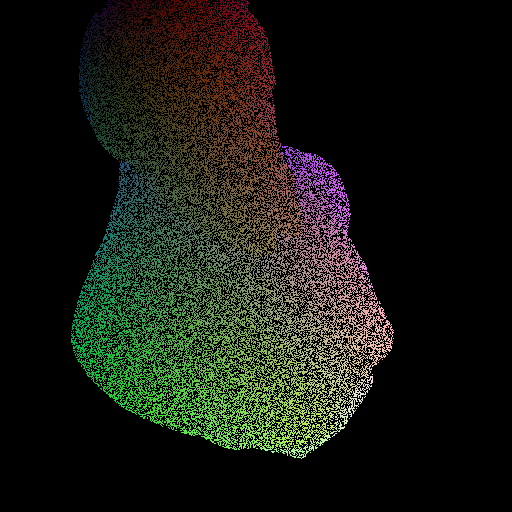
\includegraphics[width=.25\textwidth]{./Figures/train-input.png}};
		
		\draw [arrow] (oplus) -- (output);
		\draw [arrow] (sigmoid) |- (oplus);
		\draw [arrow] (LeakyReLU) -- (oplus);
		\draw [arrow] (conv2) --  node [text width=2.5cm, midway, right=1em]{LeakyReLU} (LeakyReLU);
		\draw [arrow] (conv1) --  node [text width=2.5cm, midway, right=1em]{Sigmoid} (sigmoid);
		\draw [arrow] (input) -|  node [text width=2.5cm, midway, below=1em]{Conv2D} (conv1);
		\draw [arrow] (input) -- node [text width=2.5cm, midway, right=1em]{Conv2D} (conv2);
	\end{tikzpicture}
	\caption{Gated Convolution Layer, where $ \oplus $ denotes element-wise multiplication.}
	\label{fig:gconvLayer}
\end{figure}

%\section{Canny Edge Detection for Detail Enhancement}
%The inaccuracy part is usually concentrate in the coarse surface or drastic changed surface parts of the object. The corresponding part can be extracted separately via edge detector algorithms, like Canny Edge detector. Feed the edges to a special net for normal prediction might improve the accuracy further. 

\subsection{Architecture}
\label{sec:architecture}
Based on the implementation mentioned above, the architecture roughly follows on UNet proposed by \cite{unet}, as shown in Figure \ref{fig:gcnn-archi}. 

Instead of using pooling layers for down/up samplings, gated convolution layer with stride $ (2,2) $ is used. The gated convolution using Sigmoid function for gating layer and LeakyReLU function for feature layer. All the layers are gated convolution layer with the exception of last two layer, which instead uses standard convolution layer to scale the output in range $\left[-1, 1\right]$. Other than the last two layers which use $ 1\times 1 $ kernels, all the gated convolution layer use $ 3\times 3 $ kernels with $ 1\times1 $ padding. 

The input is 3D vertex with size $ 512\times512\times3 $, and output is $ 512\times512\times3 $ normal map, which has the same resolution. There are 3 times downsamplings, each scale with 3 gated convolution layers, the third layer has stride-2. The upsampling part interpolate the feature maps 3 times with 1 gated convolution layer in each scale. 

It keeps the skip connection in UNet to remain the fine detail features. 
 
% GCNN Architecture
\begin{figure}[!h]
	\centering
	%% https://tex.stackexchange.com/questions/12020/what-is-the-easiest-way-to-draw-a-3d-cube-with-tikz
	\begin{tikzpicture}
		%% -------------------------------------- parameters ------------------------------------------------
		\pgfmathsetmacro{\vdist}{0.4}
		
		\pgfmathsetmacro{\boxsizea}{3}	%% width 512
		\pgfmathsetmacro{\boxsizeb}{1.5}	%% width 256
		\pgfmathsetmacro{\boxsizec}{1}	%% width 128
		\pgfmathsetmacro{\boxsized}{0.7}	%% width 64
		
		
		\pgfmathsetmacro{\boxwidthd}{0.1}	%% width 1
		\pgfmathsetmacro{\boxwidtha}{0.2}	%% width 3
		\pgfmathsetmacro{\boxwidthb}{\boxwidtha*1.3}	%% width 32
		\pgfmathsetmacro{\boxwidthc}{\boxwidtha*3}		%% width 64
		
		\pgfmathsetmacro{\convwshift}{9}
		\pgfmathsetmacro{\preprocessingshift}{4}
		\pgfmathsetmacro{\labelshift}{1.5}
		\pgfmathsetmacro{\gconvwshift}{0}
		
		\pgfmathsetmacro{\secrowshift}{-6}
		
		\pgfmathsetmacro{\convrowstart}{4}
		\pgfmathsetmacro{\secondrowstart}{4}
		
		%% https://www.tug.org/pracjourn/2007-4/walden/color.pdf
		\definecolor{gconvcolor}{rgb}{0.5,0.7,0.7}
		\definecolor{convcolor}{rgb}{0.5,0.7,0.3}
		\definecolor{gconvdilatedcolor}{rgb}{0.6,0,0.3}
		
		
		%% ---------------------------------- preprocessing --------------------------------------------
		%%  img_in 1x512x512
		\pgfmathsetmacro{\disttimes}{3.5}
		\pgfmathsetmacro{\yschift}{\preprocessingshift}
		\node[inner sep=0pt] (depthmap) at (\vdist*\disttimes,\yschift)
		{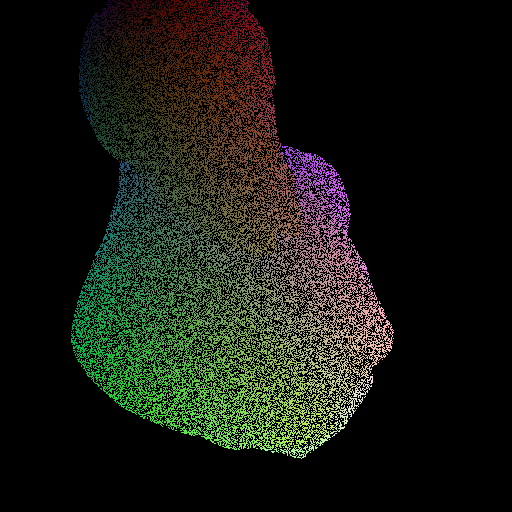
\includegraphics[width=.15\textwidth]{./Figures/train-input.png}};
		\node[text width=3.5cm] at (\vdist*\disttimes+1,\yschift-1.5) {3D Vertex};
		
		\draw [-stealth](1.45,\yschift-1.8) -- (1.45,\yschift-2.6);
		
		\draw [-stealth]  (\vdist*\disttimes+1.6,\yschift) -- (\vdist*\disttimes+1.1,\yschift);
		
		\pgfmathsetmacro{\disttimes}{10}
		\pgfmathsetmacro{\yschift}{\preprocessingshift}
		\node[inner sep=0pt] (depthmap) at (\vdist*\disttimes,\yschift)
		{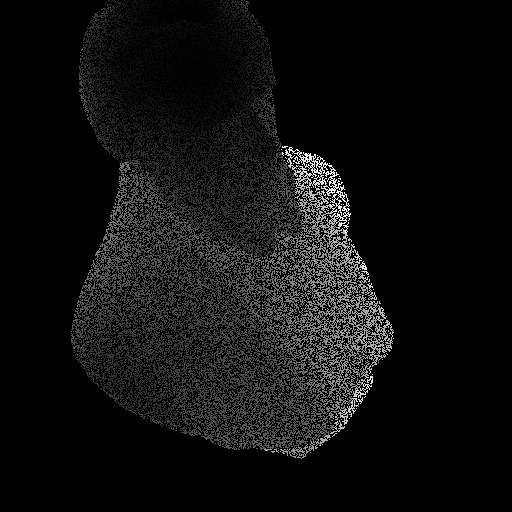
\includegraphics[width=.15\textwidth]{./Figures/train-depth-noise}};
		\node[text width=3.5cm] at (\vdist*\disttimes+1,\yschift-1.5) {Add Noise};
		
		\draw [-stealth] (\vdist*\disttimes+1.6,\yschift) -- (\vdist*\disttimes+1.1,\yschift);
		
		\pgfmathsetmacro{\disttimes}{16.5}
		\pgfmathsetmacro{\yschift}{\preprocessingshift}
		\node[inner sep=0pt] (depthmap) at (\vdist*\disttimes,\yschift)
		{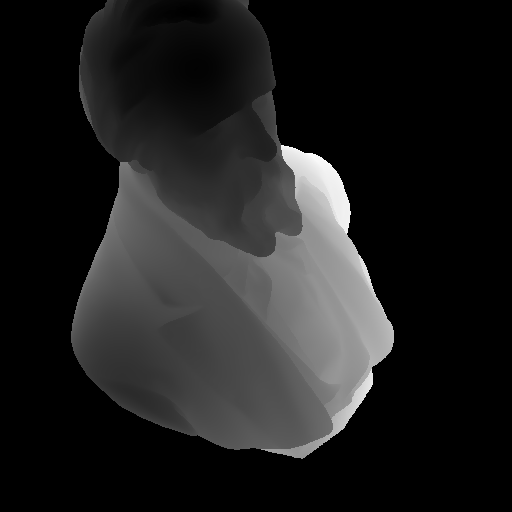
\includegraphics[width=.15\textwidth]{./Figures/train-depth.png}};
		\node[text width=2cm] at (\vdist*\disttimes+0.2,\yschift-1.5) {Depth Map};
		
		
		%% ----------------------------------- output normal map -------------------------------------
		\pgfmathsetmacro{\disttimes}{25}
		\pgfmathsetmacro{\yschift}{\preprocessingshift}
		\node[inner sep=0pt] (depthmap) at (\vdist*\disttimes,\yschift)
		{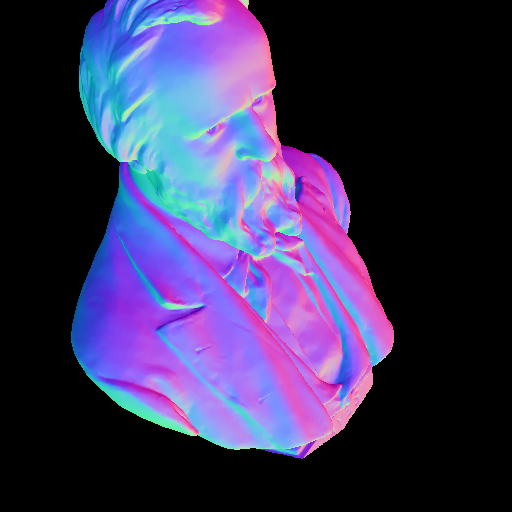
\includegraphics[width=.15\textwidth]{./Figures/train-normal-gt.png}};
		\node[text width=2.5cm] at (\vdist*\disttimes,\yschift-1.5) {Normal Map};
		
		\draw [-stealth] (\vdist*\disttimes+0.2,\yschift-2.7) -- (\vdist*\disttimes+0.2,\yschift-1.8);
		
		
		%% ------------------------------------------- vertex input ----------------------------------------------
		%% 	d_in							3x512x512
		%%	dconv1: 	d_in-->x1 			32x512x512
		\pgfmathsetmacro{\disttimes}{1}	%% width 32
		\pgfmathsetmacro{\boxsize}{\boxsizea}	%% size 512
		\pgfmathsetmacro{\boxwidth}{\boxwidthb}	%% width 32
		\pgfmathsetmacro{\yschift}{\gconvwshift}
		\node[text width=1cm] at (\vdist*\disttimes+0.1,\yschift-3.5) {32};
		\draw[black, fill=gconvcolor] (\vdist*\disttimes,\yschift,0) -- ++(-\boxwidth,0,0) -- ++(0,-\boxsize,0) -- ++(\boxwidth,0,0) -- cycle;
		\draw[black, fill=gconvcolor] (\vdist*\disttimes,\yschift,0) -- ++(0,0,-\boxsize) -- ++(0,-\boxsize,0) -- ++(0,0,\boxsize) -- cycle;
		\draw[black, fill=gconvcolor] (\vdist*\disttimes,\yschift,0) -- ++(-\boxwidth,0,0) -- ++(0,0,-\boxsize) -- ++(\boxwidth,0,0) -- cycle;
		
		%%	dconv2:		x1-->x1				32x512x512
		\pgfmathsetmacro{\disttimes}{2}	%% width 32
		\pgfmathsetmacro{\boxsize}{\boxsizea}	%% size 512
		\pgfmathsetmacro{\boxwidth}{\boxwidthb}	%% width 32
		\pgfmathsetmacro{\yschift}{\gconvwshift}
		\draw[black, fill=gconvcolor] (\vdist*\disttimes,\yschift,0) -- ++(-\boxwidth,0,0) -- ++(0,-\boxsize,0) -- ++(\boxwidth,0,0) -- cycle;
		\draw[black, fill=gconvcolor] (\vdist*\disttimes,\yschift,0) -- ++(0,0,-\boxsize) -- ++(0,-\boxsize,0) -- ++(0,0,\boxsize) -- cycle;
		\draw[black, fill=gconvcolor] (\vdist*\disttimes,\yschift,0) -- ++(-\boxwidth,0,0) -- ++(0,0,-\boxsize) -- ++(\boxwidth,0,0) -- cycle;
		
		%%	dconv3:		x1-->x1				32x512x512
		\pgfmathsetmacro{\disttimes}{3}	%% width 32
		\pgfmathsetmacro{\boxsize}{\boxsizea}	%% size 512
		\pgfmathsetmacro{\boxwidth}{\boxwidthb}	%% width 32
		\pgfmathsetmacro{\yschift}{\gconvwshift}
		\draw[black, fill=gconvcolor] (\vdist*\disttimes,\yschift,0) -- ++(-\boxwidth,0,0) -- ++(0,-\boxsize,0) -- ++(\boxwidth,0,0) -- cycle;
		\draw[black, fill=gconvcolor] (\vdist*\disttimes,\yschift,0) -- ++(0,0,-\boxsize) -- ++(0,-\boxsize,0) -- ++(0,0,\boxsize) -- cycle;
		\draw[black, fill=gconvcolor] (\vdist*\disttimes,\yschift,0) -- ++(-\boxwidth,0,0) -- ++(0,0,-\boxsize) -- ++(\boxwidth,0,0) -- cycle;
		
		\draw (\vdist*\disttimes-0.2,\yschift-3.2) -- (\vdist*\disttimes-0.2,\yschift-4);
		\draw (\vdist*\disttimes-0.2,\yschift-4) -- (\vdist*\disttimes+6.5,\yschift-4);
		\draw [-stealth] (\vdist*\disttimes+6.5,\yschift-4) -- (\vdist*\disttimes+6.5,\yschift-3.2);
		
		
		%% downsample 1
		%%	dconv4:		x1-->x2				32x256x256
		\pgfmathsetmacro{\disttimes}{4}	%% width 32
		\pgfmathsetmacro{\boxsize}{\boxsizeb}	%% size 256
		\pgfmathsetmacro{\boxwidth}{\boxwidthb}	%% width 32
		\pgfmathsetmacro{\yschift}{\gconvwshift-0.5}	%% width 32
		\draw[black, fill=gconvcolor] (\vdist*\disttimes,\yschift,0) -- ++(-\boxwidth,0,0) -- ++(0,-\boxsize,0) -- ++(\boxwidth,0,0) -- cycle;
		\draw[black, fill=gconvcolor] (\vdist*\disttimes,\yschift,0) -- ++(0,0,-\boxsize) -- ++(0,-\boxsize,0) -- ++(0,0,\boxsize) -- cycle;
		\draw[black, fill=gconvcolor] (\vdist*\disttimes,\yschift,0) -- ++(-\boxwidth,0,0) -- ++(0,0,-\boxsize) -- ++(\boxwidth,0,0) -- cycle;
		%%	dconv2:		x2-->x2				32x256x256
		\pgfmathsetmacro{\disttimes}{5}	%% width 32
		\pgfmathsetmacro{\boxsize}{\boxsizeb}	%% size 256
		\pgfmathsetmacro{\boxwidth}{\boxwidthb}	%% width 32
		\pgfmathsetmacro{\yschift}{\gconvwshift-0.5}	%% width 32
		\draw[black, fill=gconvcolor] (\vdist*\disttimes,\yschift,0) -- ++(-\boxwidth,0,0) -- ++(0,-\boxsize,0) -- ++(\boxwidth,0,0) -- cycle;
		\draw[black, fill=gconvcolor] (\vdist*\disttimes,\yschift,0) -- ++(0,0,-\boxsize) -- ++(0,-\boxsize,0) -- ++(0,0,\boxsize) -- cycle;
		\draw[black, fill=gconvcolor] (\vdist*\disttimes,\yschift,0) -- ++(-\boxwidth,0,0) -- ++(0,0,-\boxsize) -- ++(\boxwidth,0,0) -- cycle;
		%%	dconv3:		x2-->x2				32x256x256
		\pgfmathsetmacro{\disttimes}{6}	%% width 32
		\pgfmathsetmacro{\boxsize}{\boxsizeb}	%% size 256
		\pgfmathsetmacro{\boxwidth}{\boxwidthb}	%% width 32
		\pgfmathsetmacro{\yschift}{\gconvwshift-0.5}	%% width 32
		\draw[black, fill=gconvcolor] (\vdist*\disttimes,\yschift,0) -- ++(-\boxwidth,0,0) -- ++(0,-\boxsize,0) -- ++(\boxwidth,0,0) -- cycle;
		\draw[black, fill=gconvcolor] (\vdist*\disttimes,\yschift,0) -- ++(0,0,-\boxsize) -- ++(0,-\boxsize,0) -- ++(0,0,\boxsize) -- cycle;
		\draw[black, fill=gconvcolor] (\vdist*\disttimes,\yschift,0) -- ++(-\boxwidth,0,0) -- ++(0,0,-\boxsize) -- ++(\boxwidth,0,0) -- cycle;
		
		\draw (\vdist*\disttimes-0.1,\yschift-1.6) -- (\vdist*\disttimes-0.1,\yschift-2.7);
		\draw (\vdist*\disttimes-0.1,\yschift-2.7) -- (\vdist*\disttimes+4.2,\yschift-2.7);
		\draw [-stealth] (\vdist*\disttimes+4.2,\yschift-2.7) -- (\vdist*\disttimes+4.2,\yschift-1.7);
		
		
		%% downsample 2
		%%	dconv4:		x2-->x3				32x128x128
		\pgfmathsetmacro{\disttimes}{7}	%% width 32
		\pgfmathsetmacro{\boxsize}{\boxsizec}	%% size 128
		\pgfmathsetmacro{\boxwidth}{\boxwidthb}	%% width 32
		\pgfmathsetmacro{\yschift}{\gconvwshift-0.8}	%% width 32
		\draw[black, fill=gconvcolor] (\vdist*\disttimes,\yschift,0) -- ++(-\boxwidth,0,0) -- ++(0,-\boxsize,0) -- ++(\boxwidth,0,0) -- cycle;
		\draw[black, fill=gconvcolor] (\vdist*\disttimes,\yschift,0) -- ++(0,0,-\boxsize) -- ++(0,-\boxsize,0) -- ++(0,0,\boxsize) -- cycle;
		\draw[black, fill=gconvcolor] (\vdist*\disttimes,\yschift,0) -- ++(-\boxwidth,0,0) -- ++(0,0,-\boxsize) -- ++(\boxwidth,0,0) -- cycle;
		%%	dconv2:		x3-->x3				32x128x128
		\pgfmathsetmacro{\disttimes}{8}	%% width 32
		\pgfmathsetmacro{\boxsize}{\boxsizec}	%% size 128
		\pgfmathsetmacro{\boxwidth}{\boxwidthb}	%% width 32
		\pgfmathsetmacro{\yschift}{\gconvwshift-0.8}	%% width 32
		\draw[black, fill=gconvcolor] (\vdist*\disttimes,\yschift,0) -- ++(-\boxwidth,0,0) -- ++(0,-\boxsize,0) -- ++(\boxwidth,0,0) -- cycle;
		\draw[black, fill=gconvcolor] (\vdist*\disttimes,\yschift,0) -- ++(0,0,-\boxsize) -- ++(0,-\boxsize,0) -- ++(0,0,\boxsize) -- cycle;
		\draw[black, fill=gconvcolor] (\vdist*\disttimes,\yschift,0) -- ++(-\boxwidth,0,0) -- ++(0,0,-\boxsize) -- ++(\boxwidth,0,0) -- cycle;
		%%	dconv3:		x3-->x3				32x128x128
		\pgfmathsetmacro{\disttimes}{9}	%% width 32
		\pgfmathsetmacro{\boxsize}{\boxsizec}	%% size 128
		\pgfmathsetmacro{\boxwidth}{\boxwidthb}	%% width 32
		\pgfmathsetmacro{\yschift}{\gconvwshift-0.8}	%% width 32
		\draw[black, fill=gconvcolor] (\vdist*\disttimes,\yschift,0) -- ++(-\boxwidth,0,0) -- ++(0,-\boxsize,0) -- ++(\boxwidth,0,0) -- cycle;
		\draw[black, fill=gconvcolor] (\vdist*\disttimes,\yschift,0) -- ++(0,0,-\boxsize) -- ++(0,-\boxsize,0) -- ++(0,0,\boxsize) -- cycle;
		\draw[black, fill=gconvcolor] (\vdist*\disttimes,\yschift,0) -- ++(-\boxwidth,0,0) -- ++(0,0,-\boxsize) -- ++(\boxwidth,0,0) -- cycle;
		
		\draw (\vdist*\disttimes-0.1,\yschift-1.2) -- (\vdist*\disttimes-0.1,\yschift-1.8);
		\draw (\vdist*\disttimes-0.1,\yschift-1.8) -- (\vdist*\disttimes+1.8,\yschift-1.8);
		\draw [-stealth] (\vdist*\disttimes+1.8,\yschift-1.8) -- (\vdist*\disttimes+1.8,\yschift-1.2);
		
		
		%% downsample 3
		%%	dconv4:		x3-->x4				32x64x64
		\pgfmathsetmacro{\disttimes}{10}
		\pgfmathsetmacro{\boxsize}{\boxsized}	%% size 64
		\pgfmathsetmacro{\boxwidth}{\boxwidthb}	%% width 32
		\pgfmathsetmacro{\yschift}{\gconvwshift-1}
		\draw[black, fill=gconvcolor] (\vdist*\disttimes,\yschift,0) -- ++(-\boxwidth,0,0) -- ++(0,-\boxsize,0) -- ++(\boxwidth,0,0) -- cycle;
		\draw[black, fill=gconvcolor] (\vdist*\disttimes,\yschift,0) -- ++(0,0,-\boxsize) -- ++(0,-\boxsize,0) -- ++(0,0,\boxsize) -- cycle;
		\draw[black, fill=gconvcolor] (\vdist*\disttimes,\yschift,0) -- ++(-\boxwidth,0,0) -- ++(0,0,-\boxsize) -- ++(\boxwidth,0,0) -- cycle;
		%%	dconv2:		x4-->x4				32x64x64
		\pgfmathsetmacro{\disttimes}{11}
		\pgfmathsetmacro{\boxsize}{\boxsized}	%% size 64
		\pgfmathsetmacro{\boxwidth}{\boxwidthb}	%% width 32
		\pgfmathsetmacro{\yschift}{\gconvwshift-1}	%% width 32
		\draw[black, fill=gconvcolor] (\vdist*\disttimes,\yschift,0) -- ++(-\boxwidth,0,0) -- ++(0,-\boxsize,0) -- ++(\boxwidth,0,0) -- cycle;
		\draw[black, fill=gconvcolor] (\vdist*\disttimes,\yschift,0) -- ++(0,0,-\boxsize) -- ++(0,-\boxsize,0) -- ++(0,0,\boxsize) -- cycle;
		\draw[black, fill=gconvcolor] (\vdist*\disttimes,\yschift,0) -- ++(-\boxwidth,0,0) -- ++(0,0,-\boxsize) -- ++(\boxwidth,0,0) -- cycle;
		%%	dconv3:		x4-->x4				32x64x64
		\pgfmathsetmacro{\disttimes}{12}
		\pgfmathsetmacro{\boxsize}{\boxsized}	%% size 64
		\pgfmathsetmacro{\boxwidth}{\boxwidthb}	%% width 32
		\pgfmathsetmacro{\yschift}{\gconvwshift-1}	%% width 32
		\draw[black, fill=gconvcolor] (\vdist*\disttimes,\yschift,0) -- ++(-\boxwidth,0,0) -- ++(0,-\boxsize,0) -- ++(\boxwidth,0,0) -- cycle;
		\draw[black, fill=gconvcolor] (\vdist*\disttimes,\yschift,0) -- ++(0,0,-\boxsize) -- ++(0,-\boxsize,0) -- ++(0,0,\boxsize) -- cycle;
		\draw[black, fill=gconvcolor] (\vdist*\disttimes,\yschift,0) -- ++(-\boxwidth,0,0) -- ++(0,0,-\boxsize) -- ++(\boxwidth,0,0) -- cycle;
		
		%		%% dilated
		%		%%	dilated1:	x4-->x4				32x64x64
		%		\pgfmathsetmacro{\disttimes}{13}
		%		\pgfmathsetmacro{\boxsize}{\boxsized}	%% size 64
		%		\pgfmathsetmacro{\boxwidth}{\boxwidthb}	%% width 32
		%		\pgfmathsetmacro{\yschift}{\gconvwshift-1}	%% width 32
		%		\draw[black, fill=gconvdilatedcolor] (\vdist*\disttimes,\yschift,0) -- ++(-\boxwidth,0,0) -- ++(0,-\boxsize,0) -- ++(\boxwidth,0,0) -- cycle;
		%		\draw[black, fill=gconvdilatedcolor] (\vdist*\disttimes,\yschift,0) -- ++(0,0,-\boxsize) -- ++(0,-\boxsize,0) -- ++(0,0,\boxsize) -- cycle;
		%		\draw[black, fill=gconvdilatedcolor] (\vdist*\disttimes,\yschift,0) -- ++(-\boxwidth,0,0) -- ++(0,0,-\boxsize) -- ++(\boxwidth,0,0) -- cycle;
		%		%%	dilated2:	x4-->x4				32x64x64
		%		\pgfmathsetmacro{\disttimes}{14}
		%		\pgfmathsetmacro{\boxsize}{\boxsized}	%% size 64
		%		\pgfmathsetmacro{\boxwidth}{\boxwidthb}	%% width 32
		%		\pgfmathsetmacro{\yschift}{\gconvwshift-1}	%% width 32
		%		\draw[black, fill=gconvdilatedcolor] (\vdist*\disttimes,\yschift,0) -- ++(-\boxwidth,0,0) -- ++(0,-\boxsize,0) -- ++(\boxwidth,0,0) -- cycle;
		%		\draw[black, fill=gconvdilatedcolor] (\vdist*\disttimes,\yschift,0) -- ++(0,0,-\boxsize) -- ++(0,-\boxsize,0) -- ++(0,0,\boxsize) -- cycle;
		%		\draw[black, fill=gconvdilatedcolor] (\vdist*\disttimes,\yschift,0) -- ++(-\boxwidth,0,0) -- ++(0,0,-\boxsize) -- ++(\boxwidth,0,0) -- cycle;
		%		%%	dilated3:	x4-->x4				32x64x64
		%		\pgfmathsetmacro{\disttimes}{15}
		%		\pgfmathsetmacro{\boxsize}{\boxsized}	%% size 64
		%		\pgfmathsetmacro{\boxwidth}{\boxwidthb}	%% width 32
		%		\pgfmathsetmacro{\yschift}{\gconvwshift-1}	%% width 32
		%		\draw[black, fill=gconvdilatedcolor] (\vdist*\disttimes,\yschift,0) -- ++(-\boxwidth,0,0) -- ++(0,-\boxsize,0) -- ++(\boxwidth,0,0) -- cycle;
		%		\draw[black, fill=gconvdilatedcolor] (\vdist*\disttimes,\yschift,0) -- ++(0,0,-\boxsize) -- ++(0,-\boxsize,0) -- ++(0,0,\boxsize) -- cycle;
		%		\draw[black, fill=gconvdilatedcolor] (\vdist*\disttimes,\yschift,0) -- ++(-\boxwidth,0,0) -- ++(0,0,-\boxsize) -- ++(\boxwidth,0,0) -- cycle;
		%		%%	dilated4:	x4-->x4				32x64x64
		%		\pgfmathsetmacro{\disttimes}{16}
		%		\pgfmathsetmacro{\boxsize}{\boxsized}	%% size 64
		%		\pgfmathsetmacro{\boxwidth}{\boxwidthb}	%% width 32
		%		\pgfmathsetmacro{\yschift}{\gconvwshift-1}	%% width 32
		%		\draw[black, fill=gconvdilatedcolor] (\vdist*\disttimes,\yschift,0) -- ++(-\boxwidth,0,0) -- ++(0,-\boxsize,0) -- ++(\boxwidth,0,0) -- cycle;
		%		\draw[black, fill=gconvdilatedcolor] (\vdist*\disttimes,\yschift,0) -- ++(0,0,-\boxsize) -- ++(0,-\boxsize,0) -- ++(0,0,\boxsize) -- cycle;
		%		\draw[black, fill=gconvdilatedcolor] (\vdist*\disttimes,\yschift,0) -- ++(-\boxwidth,0,0) -- ++(0,0,-\boxsize) -- ++(\boxwidth,0,0) -- cycle;
		%		
		%		
		%		
		%		
		%		%%	dconv2:		x4-->x4				32x64x64
		%		\pgfmathsetmacro{\disttimes}{17}
		%		\pgfmathsetmacro{\boxsize}{\boxsized}	%% size 64
		%		\pgfmathsetmacro{\boxwidth}{\boxwidthb}	%% width 32
		%		\pgfmathsetmacro{\yschift}{\gconvwshift-1}	%% width 32
		%		\draw[black, fill=gconvcolor] (\vdist*\disttimes,\yschift,0) -- ++(-\boxwidth,0,0) -- ++(0,-\boxsize,0) -- ++(\boxwidth,0,0) -- cycle;
		%		\draw[black, fill=gconvcolor] (\vdist*\disttimes,\yschift,0) -- ++(0,0,-\boxsize) -- ++(0,-\boxsize,0) -- ++(0,0,\boxsize) -- cycle;
		%		\draw[black, fill=gconvcolor] (\vdist*\disttimes,\yschift,0) -- ++(-\boxwidth,0,0) -- ++(0,0,-\boxsize) -- ++(\boxwidth,0,0) -- cycle;
		%		%%	dconv3:		x4-->x4				32x64x64
		%		\pgfmathsetmacro{\disttimes}{18}
		%		\pgfmathsetmacro{\boxsize}{\boxsized}	%% size 64
		%		\pgfmathsetmacro{\boxwidth}{\boxwidthb}	%% width 32
		%		\pgfmathsetmacro{\yschift}{\gconvwshift-1}	%% width 32
		%		\draw[black, fill=gconvcolor] (\vdist*\disttimes,\yschift,0) -- ++(-\boxwidth,0,0) -- ++(0,-\boxsize,0) -- ++(\boxwidth,0,0) -- cycle;
		%		\draw[black, fill=gconvcolor] (\vdist*\disttimes,\yschift,0) -- ++(0,0,-\boxsize) -- ++(0,-\boxsize,0) -- ++(0,0,\boxsize) -- cycle;
		%		\draw[black, fill=gconvcolor] (\vdist*\disttimes,\yschift,0) -- ++(-\boxwidth,0,0) -- ++(0,0,-\boxsize) -- ++(\boxwidth,0,0) -- cycle;
		
		
		%% ----------------------------------- upsampling -------------------------------------
		
		%% upsample 1
		%% interpolate	x4-->x3_us			64x128x128
		\pgfmathsetmacro{\disttimes}{13}
		\pgfmathsetmacro{\boxsize}{\boxsizec}	%% size 128
		\pgfmathsetmacro{\boxwidth}{\boxwidthb}	%% width 32
		\pgfmathsetmacro{\yschift}{\gconvwshift-0.9}	%% width 32
		\draw[black, fill=gconvcolor] (\vdist*\disttimes,\yschift,0) -- ++(-\boxwidth,0,0) -- ++(0,-\boxsize,0) -- ++(\boxwidth,0,0) -- cycle;
		\draw[black, fill=gconvcolor] (\vdist*\disttimes,\yschift,0) -- ++(0,0,-\boxsize) -- ++(0,-\boxsize,0) -- ++(0,0,\boxsize) -- cycle;
		\draw[black, fill=gconvcolor] (\vdist*\disttimes,\yschift,0) -- ++(-\boxwidth,0,0) -- ++(0,0,-\boxsize) -- ++(\boxwidth,0,0) -- cycle;
		
		%% concatenate x3_us
		\pgfmathsetmacro{\boxsize}{\boxsizec}	%% size 128
		\pgfmathsetmacro{\boxwidth}{\boxwidthb}	%% width 32
		\pgfmathsetmacro{\yschift}{\gconvwshift-0.9}	%% width 32
		\draw[black, fill=gconvcolor] (\vdist*\disttimes+\boxwidth,\yschift,0) -- ++(-\boxwidth,0,0) -- ++(0,-\boxsize,0) -- ++(\boxwidth,0,0) -- cycle;
		\draw[black, fill=gconvcolor] (\vdist*\disttimes+\boxwidth,\yschift,0) -- ++(0,0,-\boxsize) -- ++(0,-\boxsize,0) -- ++(0,0,\boxsize) -- cycle;
		\draw[black, fill=gconvcolor] (\vdist*\disttimes+\boxwidth,\yschift,0) -- ++(-\boxwidth,0,0) -- ++(0,0,-\boxsize) -- ++(\boxwidth,0,0) -- cycle;
		
		%% uconv1		x3_us-->x3			32x128x128
		\pgfmathsetmacro{\disttimes}{15}
		\pgfmathsetmacro{\boxsize}{\boxsizec}	%% size 128
		\pgfmathsetmacro{\boxwidth}{\boxwidthb}	%% width 32
		\pgfmathsetmacro{\yschift}{\gconvwshift-0.9}	%% width 32
		\draw[black, fill=gconvcolor] (\vdist*\disttimes,\yschift,0) -- ++(-\boxwidth,0,0) -- ++(0,-\boxsize,0) -- ++(\boxwidth,0,0) -- cycle;
		\draw[black, fill=gconvcolor] (\vdist*\disttimes,\yschift,0) -- ++(0,0,-\boxsize) -- ++(0,-\boxsize,0) -- ++(0,0,\boxsize) -- cycle;
		\draw[black, fill=gconvcolor] (\vdist*\disttimes,\yschift,0) -- ++(-\boxwidth,0,0) -- ++(0,0,-\boxsize) -- ++(\boxwidth,0,0) -- cycle;
		
		%% upsample 2
		%% interpolate	x3-->x2_us			32x256x256
		\pgfmathsetmacro{\disttimes}{16}
		\pgfmathsetmacro{\boxsize}{\boxsizeb}	%% size 256
		\pgfmathsetmacro{\boxwidth}{\boxwidthb}	%% width 32
		\pgfmathsetmacro{\yschift}{\gconvwshift-0.6}	%% width 32
		\draw[black, fill=gconvcolor] (\vdist*\disttimes,\yschift,0) -- ++(-\boxwidth,0,0) -- ++(0,-\boxsize,0) -- ++(\boxwidth,0,0) -- cycle;
		\draw[black, fill=gconvcolor] (\vdist*\disttimes,\yschift,0) -- ++(0,0,-\boxsize) -- ++(0,-\boxsize,0) -- ++(0,0,\boxsize) -- cycle;
		\draw[black, fill=gconvcolor] (\vdist*\disttimes,\yschift,0) -- ++(-\boxwidth,0,0) -- ++(0,0,-\boxsize) -- ++(\boxwidth,0,0) -- cycle;
		%% concatenated x2
		\pgfmathsetmacro{\boxsize}{\boxsizeb}	%% size 256
		\pgfmathsetmacro{\boxwidth}{\boxwidthb}	%% width 32
		\pgfmathsetmacro{\yschift}{\gconvwshift-0.6}	%% width 32
		\draw[black, fill=gconvcolor] (\vdist*\disttimes+\boxwidth,\yschift,0) -- ++(-\boxwidth,0,0) -- ++(0,-\boxsize,0) -- ++(\boxwidth,0,0) -- cycle;
		\draw[black, fill=gconvcolor] (\vdist*\disttimes+\boxwidth,\yschift,0) -- ++(0,0,-\boxsize) -- ++(0,-\boxsize,0) -- ++(0,0,\boxsize) -- cycle;
		\draw[black, fill=gconvcolor] (\vdist*\disttimes+\boxwidth,\yschift,0) -- ++(-\boxwidth,0,0) -- ++(0,0,-\boxsize) -- ++(\boxwidth,0,0) -- cycle;
		
		%% uconv2 		x2,x2_us-->x2		32x256x256
		\pgfmathsetmacro{\disttimes}{18}
		\pgfmathsetmacro{\boxsize}{\boxsizeb}	%% size 256
		\pgfmathsetmacro{\boxwidth}{\boxwidthb}	%% width 32
		\pgfmathsetmacro{\yschift}{\gconvwshift-0.6}	%% width 32
		\draw[black, fill=gconvcolor] (\vdist*\disttimes,\yschift,0) -- ++(-\boxwidth,0,0) -- ++(0,-\boxsize,0) -- ++(\boxwidth,0,0) -- cycle;
		\draw[black, fill=gconvcolor] (\vdist*\disttimes,\yschift,0) -- ++(0,0,-\boxsize) -- ++(0,-\boxsize,0) -- ++(0,0,\boxsize) -- cycle;
		\draw[black, fill=gconvcolor] (\vdist*\disttimes,\yschift,0) -- ++(-\boxwidth,0,0) -- ++(0,0,-\boxsize) -- ++(\boxwidth,0,0) -- cycle;
		
		
		%% upsample 3
		%% interpolate	x2-->x1_us			32x512x512
		\pgfmathsetmacro{\disttimes}{19}
		\pgfmathsetmacro{\boxsize}{\boxsizea}	%% size 512
		\pgfmathsetmacro{\boxwidth}{\boxwidthb}	%% width 32
		\pgfmathsetmacro{\yschift}{\gconvwshift}	%% width 32
		\draw[black, fill=gconvcolor] (\vdist*\disttimes,\yschift,0) -- ++(-\boxwidth,0,0) -- ++(0,-\boxsize,0) -- ++(\boxwidth,0,0) -- cycle;
		\draw[black, fill=gconvcolor] (\vdist*\disttimes,\yschift,0) -- ++(0,0,-\boxsize) -- ++(0,-\boxsize,0) -- ++(0,0,\boxsize) -- cycle;
		\draw[black, fill=gconvcolor] (\vdist*\disttimes,\yschift,0) -- ++(-\boxwidth,0,0) -- ++(0,0,-\boxsize) -- ++(\boxwidth,0,0) -- cycle;
		%% concatenated x1 and x1_us
		\pgfmathsetmacro{\boxsize}{\boxsizea}	%% size 512
		\pgfmathsetmacro{\boxwidth}{\boxwidthb}	%% width 32
		\pgfmathsetmacro{\yschift}{\gconvwshift}	%% width 32
		\draw[black, fill=gconvcolor] (\vdist*\disttimes+\boxwidth,\yschift,0) -- ++(-\boxwidth,0,0) -- ++(0,-\boxsize,0) -- ++(\boxwidth,0,0) -- cycle;
		\draw[black, fill=gconvcolor] (\vdist*\disttimes+\boxwidth,\yschift,0) -- ++(0,0,-\boxsize) -- ++(0,-\boxsize,0) -- ++(0,0,\boxsize) -- cycle;
		\draw[black, fill=gconvcolor] (\vdist*\disttimes+\boxwidth,\yschift,0) -- ++(-\boxwidth,0,0) -- ++(0,0,-\boxsize) -- ++(\boxwidth,0,0) -- cycle;
		
		
		%% uconv3		x1,x1_us-->x1		32x512x512
		\pgfmathsetmacro{\disttimes}{21}
		\pgfmathsetmacro{\boxsize}{\boxsizea}	%% size 512
		\pgfmathsetmacro{\boxwidth}{\boxwidthb}	%% width 32
		\pgfmathsetmacro{\yschift}{\gconvwshift}	%% width 32
		\draw[black, fill=gconvcolor] (\vdist*\disttimes,\yschift,0) -- ++(-\boxwidth,0,0) -- ++(0,-\boxsize,0) -- ++(\boxwidth,0,0) -- cycle;
		\draw[black, fill=gconvcolor] (\vdist*\disttimes,\yschift,0) -- ++(0,0,-\boxsize) -- ++(0,-\boxsize,0) -- ++(0,0,\boxsize) -- cycle;
		\draw[black, fill=gconvcolor] (\vdist*\disttimes,\yschift,0) -- ++(-\boxwidth,0,0) -- ++(0,0,-\boxsize) -- ++(\boxwidth,0,0) -- cycle;
		
		%% conv1		x1-->xout			3x512x512
		\pgfmathsetmacro{\disttimes}{22}
		\pgfmathsetmacro{\boxsize}{\boxsizea}	%% size 512
		\pgfmathsetmacro{\boxwidth}{\boxwidthb}	%% width 3
		\pgfmathsetmacro{\yschift}{\gconvwshift}	%% width 32
		\node[text width=1cm] at (\vdist*\disttimes+0.2,\yschift-3.3) {32};
		\draw[black, fill=convcolor] (\vdist*\disttimes,\yschift,0) -- ++(-\boxwidth,0,0) -- ++(0,-\boxsize,0) -- ++(\boxwidth,0,0) -- cycle;
		\draw[black, fill=convcolor] (\vdist*\disttimes,\yschift,0) -- ++(0,0,-\boxsize) -- ++(0,-\boxsize,0) -- ++(0,0,\boxsize) -- cycle;
		\draw[black, fill=convcolor] (\vdist*\disttimes,\yschift,0) -- ++(-\boxwidth,0,0) -- ++(0,0,-\boxsize) -- ++(\boxwidth,0,0) -- cycle;
		
		
		
		%% conv2		xout-->xout			3x512x512
		\pgfmathsetmacro{\disttimes}{23}
		\pgfmathsetmacro{\boxsize}{\boxsizea}	%% size 512
		\pgfmathsetmacro{\boxwidth}{\boxwidthd}	%% width 3
		\pgfmathsetmacro{\yschift}{\gconvwshift}	%% width 32
		\node[text width=1cm] at (\vdist*\disttimes+0.5,\yschift-3.3) {3};
		\draw[black, fill=convcolor] (\vdist*\disttimes,\yschift,0) -- ++(-\boxwidth,0,0) -- ++(0,-\boxsize,0) -- ++(\boxwidth,0,0) -- cycle;
		\draw[black, fill=convcolor] (\vdist*\disttimes,\yschift,0) -- ++(0,0,-\boxsize) -- ++(0,-\boxsize,0) -- ++(0,0,\boxsize) -- cycle;
		\draw[black, fill=convcolor] (\vdist*\disttimes,\yschift,0) -- ++(-\boxwidth,0,0) -- ++(0,0,-\boxsize) -- ++(\boxwidth,0,0) -- cycle;
		
		
		%% ------------------------------------- label ----------------------------------------------		
		\pgfmathsetmacro{\disttimes}{10}
		\pgfmathsetmacro{\boxsize}{\boxsized}	%% size 512
		\pgfmathsetmacro{\boxwidth}{\boxwidthc}	%% width 3
		\pgfmathsetmacro{\yschift}{\labelshift}	%% width 32
		\node[text width=3.5cm] at (\vdist*\disttimes+1,\yschift-1) {Conv2d};
		\draw[black, fill=convcolor] (\vdist*\disttimes,\yschift,0) -- ++(-\boxwidth,0,0) -- ++(0,-\boxsize,0) -- ++(\boxwidth,0,0) -- cycle;
		\draw[black, fill=convcolor] (\vdist*\disttimes,\yschift,0) -- ++(0,0,-\boxsize) -- ++(0,-\boxsize,0) -- ++(0,0,\boxsize) -- cycle;
		\draw[black, fill=convcolor] (\vdist*\disttimes,\yschift,0) -- ++(-\boxwidth,0,0) -- ++(0,0,-\boxsize) -- ++(\boxwidth,0,0) -- cycle;
		
		\pgfmathsetmacro{\disttimes}{15}
		\pgfmathsetmacro{\boxsize}{\boxsized}	%% size 512
		\pgfmathsetmacro{\boxwidth}{\boxwidthc}	%% width 3
		\pgfmathsetmacro{\yschift}{\labelshift}	%% width 32
		\node[text width=3.5cm] at (\vdist*\disttimes+1,\yschift-1) {Gated};
		\draw[black, fill=gconvcolor] (\vdist*\disttimes,\yschift,0) -- ++(-\boxwidth,0,0) -- ++(0,-\boxsize,0) -- ++(\boxwidth,0,0) -- cycle;
		\draw[black, fill=gconvcolor] (\vdist*\disttimes,\yschift,0) -- ++(0,0,-\boxsize) -- ++(0,-\boxsize,0) -- ++(0,0,\boxsize) -- cycle;
		\draw[black, fill=gconvcolor] (\vdist*\disttimes,\yschift,0) -- ++(-\boxwidth,0,0) -- ++(0,0,-\boxsize) -- ++(\boxwidth,0,0) -- cycle;
		
		
		
	\end{tikzpicture}
	
	\caption{Basic Normal Neural Network model based on Gated Convolution layer and UNet architecture. }
	\label{fig:gcnn-archi}
\end{figure}

\subsection{Loss Function}

\subsubsection{Perceptual Loss}

\cite{perceptual-loss} proposed perceptual loss.

\subsubsection{L2 Loss}
The loss function is based on mean square error is described as follows: 

\begin{equation}\label{gcnn-loss}
	\begin{array}{ll}
		l(x,y)= L  &= \{l_1, ..., l_N\}^T\\ 
		l_n &= mean(Mask_{ol}(x_n - y_n)^2\cdot p + (x_n - y_n)^2\cdot Mask_{nol})\\
	\end{array}
\end{equation}

where $ x $ is input, $ y $ is target, $ N $ is the batch size. $ Mask_{ol} $ is the mask for the outlier, $ p $ is the penalty of the outlier, it is set as 1.4.

\newpage
\section{Guided normal inference using GCNN}




\subsection{Image Guided normal inference}
The normal inference can be guided by a RGB or gray-scale image, since the image is captured by passive method, it is fully-dense comparing to depth map, hence provides a complete view of the scene. 
The architecture is shown in Figure \ref{fig:ng-archi}. The upper branch is the similar with GCNN model but with 4 additional concatenate layers, furthermore, 1 gated convolution layer is added before concatenate with image branch. The image branch takes a single grayscale image as input, then 3 times downsamplins with 3 standard layers in each scale. In the upsampling part, the feature map upsampled 3 times and concatenate with the last layer in the downsampling part before interpolation.


% architecture of NG
\begin{figure}[!h]
	\centering
	%% https://tex.stackexchange.com/questions/12020/what-is-the-easiest-way-to-draw-a-3d-cube-with-tikz
	\begin{tikzpicture}
		%% -------------------------------------- parameters ------------------------------------------------
		\pgfmathsetmacro{\vdist}{0.4}
		
		\pgfmathsetmacro{\boxsizea}{3}	%% width 512
		\pgfmathsetmacro{\boxsizeb}{1.5}	%% width 256
		\pgfmathsetmacro{\boxsizec}{1}	%% width 128
		\pgfmathsetmacro{\boxsized}{0.7}	%% width 64
		
		
		\pgfmathsetmacro{\boxwidthd}{0.05}	%% width 1
		\pgfmathsetmacro{\boxwidtha}{0.1}	%% width 3
		\pgfmathsetmacro{\boxwidthb}{\boxwidtha*2}	%% width 32
		\pgfmathsetmacro{\boxwidthc}{\boxwidtha*3}		%% width 64
		
		\pgfmathsetmacro{\preprocessingshift}{13}
		\pgfmathsetmacro{\labelshift}{10.5}
		\pgfmathsetmacro{\gconvwshift}{9}
		\pgfmathsetmacro{\imgshift}{3.5}
		\pgfmathsetmacro{\convwshift}{0}
		
		\pgfmathsetmacro{\secrowshift}{-6}
		
		\pgfmathsetmacro{\convrowstart}{4}
		\pgfmathsetmacro{\secondrowstart}{4}
		
		%% https://www.tug.org/pracjourn/2007-4/walden/color.pdf
		\definecolor{gconvcolor}{rgb}{0.5,0.8,0.8}
		\definecolor{convcolor}{rgb}{0.9,0.5,0.2}
		\definecolor{interpolatecolor}{rgb}{0.3,0.9,0.5}
		\definecolor{catcolor}{rgb}{0.9,0.3,0.9}
		
		%% ---------------------------------- preprocessing --------------------------------------------
		%%  img_in 1x512x512
		\pgfmathsetmacro{\disttimes}{3.5}
		\pgfmathsetmacro{\yschift}{\preprocessingshift}
		\node[inner sep=0pt] (depthmap) at (\vdist*\disttimes,\yschift)
		{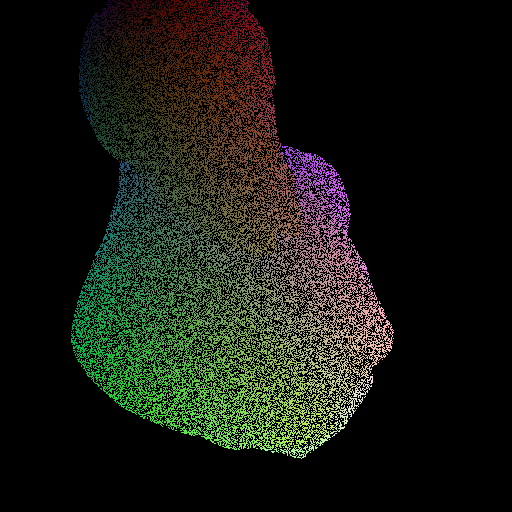
\includegraphics[width=.15\textwidth]{./Figures/train-input.png}};
		\node[text width=3.5cm] at (\vdist*\disttimes+1,\yschift-1.5) {3D Vertex};
		
		\draw [-stealth](1.45,\yschift-1.8) -- (1.45,\yschift-2.6);
		
		\draw [-stealth]  (\vdist*\disttimes+1.6,\yschift) -- (\vdist*\disttimes+1.1,\yschift);
		
		\pgfmathsetmacro{\disttimes}{10}
		\pgfmathsetmacro{\yschift}{\preprocessingshift}
		\node[inner sep=0pt] (depthmap) at (\vdist*\disttimes,\yschift)
		{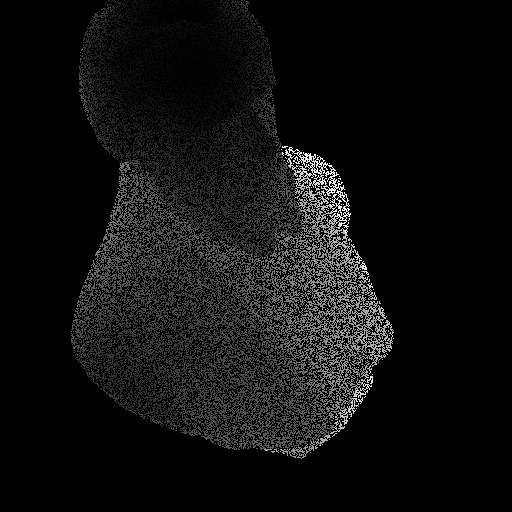
\includegraphics[width=.15\textwidth]{./Figures/train-depth-noise.png}};
		\node[text width=3.5cm] at (\vdist*\disttimes+1,\yschift-1.5) {Add Noise};
		
		\draw [-stealth] (\vdist*\disttimes+1.6,\yschift) -- (\vdist*\disttimes+1.1,\yschift);
		
		\pgfmathsetmacro{\disttimes}{16.5}
		\pgfmathsetmacro{\yschift}{\preprocessingshift}
		\node[inner sep=0pt] (depthmap) at (\vdist*\disttimes,\yschift)
		{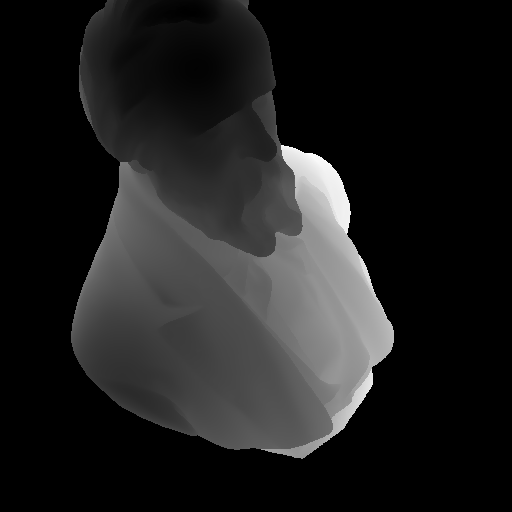
\includegraphics[width=.15\textwidth]{./Figures/train-depth.png}};
		\node[text width=2cm] at (\vdist*\disttimes+0.2,\yschift-1.5) {Depth Map};
		
		%% ------------------------------------ img preprocessing -------------------------------------
		\pgfmathsetmacro{\disttimes}{3.5}
		\pgfmathsetmacro{\yschift}{\imgshift}
		\node[inner sep=0pt] (image) at (\vdist*\disttimes,\yschift)
		{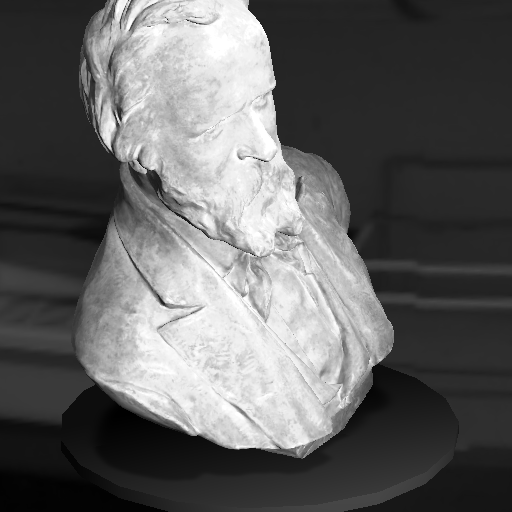
\includegraphics[width=.15\textwidth]{./Figures/train-image.png}};
		\node[text width=3.5cm] at (\vdist*\disttimes+1,\yschift-1.5) {Image};
		
		\draw [-stealth](1.45,\yschift-1.8) -- (1.45,\yschift-2.2);
		
		
		
		%% ----------------------------------- output normal map -------------------------------------
		\pgfmathsetmacro{\disttimes}{32.5}
		\pgfmathsetmacro{\yschift}{\preprocessingshift}
		\node[inner sep=0pt] (depthmap) at (\vdist*\disttimes,\yschift)
		{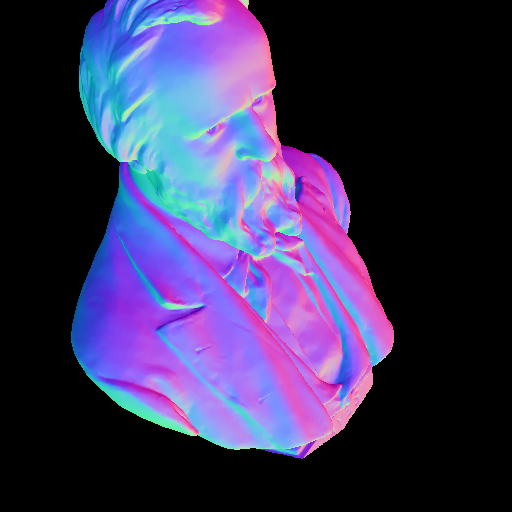
\includegraphics[width=.15\textwidth]{./Figures/train-normal-gt.png}};
		\node[text width=2.5cm] at (\vdist*\disttimes,\yschift-1.5) {Normal Map};
		
		\draw [-stealth] (\vdist*\disttimes+0.2,\yschift-2.7) -- (\vdist*\disttimes+0.2,\yschift-1.8);
		
		
		%% ------------------------------------------- vertex input ----------------------------------------------
		%% 	d_in							3x512x512
		%%	dconv1: 	d_in-->x1 			32x512x512
		\pgfmathsetmacro{\disttimes}{1}	%% width 32
		\pgfmathsetmacro{\boxsize}{\boxsizea}	%% size 512
		\pgfmathsetmacro{\boxwidth}{\boxwidthb}	%% width 32
		\pgfmathsetmacro{\yschift}{\gconvwshift}
		\node[text width=1cm] at (\vdist*\disttimes+0.1,\yschift-3.5) {32};
		\draw[black, fill=gconvcolor] (\vdist*\disttimes,\yschift,0) -- ++(-\boxwidth,0,0) -- ++(0,-\boxsize,0) -- ++(\boxwidth,0,0) -- cycle;
		\draw[black, fill=gconvcolor] (\vdist*\disttimes,\yschift,0) -- ++(0,0,-\boxsize) -- ++(0,-\boxsize,0) -- ++(0,0,\boxsize) -- cycle;
		\draw[black, fill=gconvcolor] (\vdist*\disttimes,\yschift,0) -- ++(-\boxwidth,0,0) -- ++(0,0,-\boxsize) -- ++(\boxwidth,0,0) -- cycle;
		
		%%	dconv2:		x1-->x1				32x512x512
		\pgfmathsetmacro{\disttimes}{2}	%% width 32
		\pgfmathsetmacro{\boxsize}{\boxsizea}	%% size 512
		\pgfmathsetmacro{\boxwidth}{\boxwidthb}	%% width 32
		\pgfmathsetmacro{\yschift}{\gconvwshift}
		\draw[black, fill=gconvcolor] (\vdist*\disttimes,\yschift,0) -- ++(-\boxwidth,0,0) -- ++(0,-\boxsize,0) -- ++(\boxwidth,0,0) -- cycle;
		\draw[black, fill=gconvcolor] (\vdist*\disttimes,\yschift,0) -- ++(0,0,-\boxsize) -- ++(0,-\boxsize,0) -- ++(0,0,\boxsize) -- cycle;
		\draw[black, fill=gconvcolor] (\vdist*\disttimes,\yschift,0) -- ++(-\boxwidth,0,0) -- ++(0,0,-\boxsize) -- ++(\boxwidth,0,0) -- cycle;
		
		%%	dconv3:		x1-->x1				32x512x512
		\pgfmathsetmacro{\disttimes}{3}	%% width 32
		\pgfmathsetmacro{\boxsize}{\boxsizea}	%% size 512
		\pgfmathsetmacro{\boxwidth}{\boxwidthb}	%% width 32
		\pgfmathsetmacro{\yschift}{\gconvwshift}
		\draw[black, fill=gconvcolor] (\vdist*\disttimes,\yschift,0) -- ++(-\boxwidth,0,0) -- ++(0,-\boxsize,0) -- ++(\boxwidth,0,0) -- cycle;
		\draw[black, fill=gconvcolor] (\vdist*\disttimes,\yschift,0) -- ++(0,0,-\boxsize) -- ++(0,-\boxsize,0) -- ++(0,0,\boxsize) -- cycle;
		\draw[black, fill=gconvcolor] (\vdist*\disttimes,\yschift,0) -- ++(-\boxwidth,0,0) -- ++(0,0,-\boxsize) -- ++(\boxwidth,0,0) -- cycle;
		
		\draw (\vdist*\disttimes-0.1,\yschift-3) -- (\vdist*\disttimes-0.1,\yschift-3.7);
		\draw (\vdist*\disttimes-0.1,\yschift-3.7) -- (\vdist*\disttimes+9.2,\yschift-3.7);
		\draw [-stealth] (\vdist*\disttimes+9.2,\yschift-3.7) -- (\vdist*\disttimes+9.2,\yschift-3);
		
		%% downsample 1
		%%	dconv4:		x1-->x2				32x256x256
		\pgfmathsetmacro{\disttimes}{4}	%% width 32
		\pgfmathsetmacro{\boxsize}{\boxsizeb}	%% size 256
		\pgfmathsetmacro{\boxwidth}{\boxwidthb}	%% width 32
		\pgfmathsetmacro{\yschift}{\gconvwshift-0.5}	%% width 32
		\draw[black, fill=gconvcolor] (\vdist*\disttimes,\yschift,0) -- ++(-\boxwidth,0,0) -- ++(0,-\boxsize,0) -- ++(\boxwidth,0,0) -- cycle;
		\draw[black, fill=gconvcolor] (\vdist*\disttimes,\yschift,0) -- ++(0,0,-\boxsize) -- ++(0,-\boxsize,0) -- ++(0,0,\boxsize) -- cycle;
		\draw[black, fill=gconvcolor] (\vdist*\disttimes,\yschift,0) -- ++(-\boxwidth,0,0) -- ++(0,0,-\boxsize) -- ++(\boxwidth,0,0) -- cycle;
		%%	dconv2:		x2-->x2				32x256x256
		\pgfmathsetmacro{\disttimes}{5}	%% width 32
		\pgfmathsetmacro{\boxsize}{\boxsizeb}	%% size 256
		\pgfmathsetmacro{\boxwidth}{\boxwidthb}	%% width 32
		\pgfmathsetmacro{\yschift}{\gconvwshift-0.5}	%% width 32
		\draw[black, fill=gconvcolor] (\vdist*\disttimes,\yschift,0) -- ++(-\boxwidth,0,0) -- ++(0,-\boxsize,0) -- ++(\boxwidth,0,0) -- cycle;
		\draw[black, fill=gconvcolor] (\vdist*\disttimes,\yschift,0) -- ++(0,0,-\boxsize) -- ++(0,-\boxsize,0) -- ++(0,0,\boxsize) -- cycle;
		\draw[black, fill=gconvcolor] (\vdist*\disttimes,\yschift,0) -- ++(-\boxwidth,0,0) -- ++(0,0,-\boxsize) -- ++(\boxwidth,0,0) -- cycle;
		%%	dconv3:		x2-->x2				32x256x256
		\pgfmathsetmacro{\disttimes}{6}	%% width 32
		\pgfmathsetmacro{\boxsize}{\boxsizeb}	%% size 256
		\pgfmathsetmacro{\boxwidth}{\boxwidthb}	%% width 32
		\pgfmathsetmacro{\yschift}{\gconvwshift-0.5}	%% width 32
		\draw[black, fill=gconvcolor] (\vdist*\disttimes,\yschift,0) -- ++(-\boxwidth,0,0) -- ++(0,-\boxsize,0) -- ++(\boxwidth,0,0) -- cycle;
		\draw[black, fill=gconvcolor] (\vdist*\disttimes,\yschift,0) -- ++(0,0,-\boxsize) -- ++(0,-\boxsize,0) -- ++(0,0,\boxsize) -- cycle;
		\draw[black, fill=gconvcolor] (\vdist*\disttimes,\yschift,0) -- ++(-\boxwidth,0,0) -- ++(0,0,-\boxsize) -- ++(\boxwidth,0,0) -- cycle;
		
		\draw (\vdist*\disttimes-0.1,\yschift-1.6) -- (\vdist*\disttimes-0.1,\yschift-2.7);
		\draw (\vdist*\disttimes-0.1,\yschift-2.7) -- (\vdist*\disttimes+6,\yschift-2.7);
		\draw [-stealth] (\vdist*\disttimes+6,\yschift-2.7) -- (\vdist*\disttimes+6,\yschift-1.7);
		
		
		%% downsample 2
		%%	dconv4:		x2-->x3				32x128x128
		\pgfmathsetmacro{\disttimes}{7}	%% width 32
		\pgfmathsetmacro{\boxsize}{\boxsizec}	%% size 128
		\pgfmathsetmacro{\boxwidth}{\boxwidthb}	%% width 32
		\pgfmathsetmacro{\yschift}{\gconvwshift-0.8}	%% width 32
		\draw[black, fill=gconvcolor] (\vdist*\disttimes,\yschift,0) -- ++(-\boxwidth,0,0) -- ++(0,-\boxsize,0) -- ++(\boxwidth,0,0) -- cycle;
		\draw[black, fill=gconvcolor] (\vdist*\disttimes,\yschift,0) -- ++(0,0,-\boxsize) -- ++(0,-\boxsize,0) -- ++(0,0,\boxsize) -- cycle;
		\draw[black, fill=gconvcolor] (\vdist*\disttimes,\yschift,0) -- ++(-\boxwidth,0,0) -- ++(0,0,-\boxsize) -- ++(\boxwidth,0,0) -- cycle;
		%%	dconv2:		x3-->x3				32x128x128
		\pgfmathsetmacro{\disttimes}{8}	%% width 32
		\pgfmathsetmacro{\boxsize}{\boxsizec}	%% size 128
		\pgfmathsetmacro{\boxwidth}{\boxwidthb}	%% width 32
		\pgfmathsetmacro{\yschift}{\gconvwshift-0.8}	%% width 32
		\draw[black, fill=gconvcolor] (\vdist*\disttimes,\yschift,0) -- ++(-\boxwidth,0,0) -- ++(0,-\boxsize,0) -- ++(\boxwidth,0,0) -- cycle;
		\draw[black, fill=gconvcolor] (\vdist*\disttimes,\yschift,0) -- ++(0,0,-\boxsize) -- ++(0,-\boxsize,0) -- ++(0,0,\boxsize) -- cycle;
		\draw[black, fill=gconvcolor] (\vdist*\disttimes,\yschift,0) -- ++(-\boxwidth,0,0) -- ++(0,0,-\boxsize) -- ++(\boxwidth,0,0) -- cycle;
		%%	dconv3:		x3-->x3				32x128x128
		\pgfmathsetmacro{\disttimes}{9}	%% width 32
		\pgfmathsetmacro{\boxsize}{\boxsizec}	%% size 128
		\pgfmathsetmacro{\boxwidth}{\boxwidthb}	%% width 32
		\pgfmathsetmacro{\yschift}{\gconvwshift-0.8}	%% width 32
		\draw[black, fill=gconvcolor] (\vdist*\disttimes,\yschift,0) -- ++(-\boxwidth,0,0) -- ++(0,-\boxsize,0) -- ++(\boxwidth,0,0) -- cycle;
		\draw[black, fill=gconvcolor] (\vdist*\disttimes,\yschift,0) -- ++(0,0,-\boxsize) -- ++(0,-\boxsize,0) -- ++(0,0,\boxsize) -- cycle;
		\draw[black, fill=gconvcolor] (\vdist*\disttimes,\yschift,0) -- ++(-\boxwidth,0,0) -- ++(0,0,-\boxsize) -- ++(\boxwidth,0,0) -- cycle;
		
		\draw (\vdist*\disttimes-0.1,\yschift-1.2) -- (\vdist*\disttimes-0.1,\yschift-1.8);
		\draw (\vdist*\disttimes-0.1,\yschift-1.8) -- (\vdist*\disttimes+2.8,\yschift-1.8);
		\draw [-stealth] (\vdist*\disttimes+2.8,\yschift-1.8) -- (\vdist*\disttimes+2.8,\yschift-1.2);
		
		
		%% downsample 3
		%%	dconv4:		x3-->x4				32x64x64
		\pgfmathsetmacro{\disttimes}{10}
		\pgfmathsetmacro{\boxsize}{\boxsized}	%% size 64
		\pgfmathsetmacro{\boxwidth}{\boxwidthb}	%% width 32
		\pgfmathsetmacro{\yschift}{\gconvwshift-1}
		\draw[black, fill=gconvcolor] (\vdist*\disttimes,\yschift,0) -- ++(-\boxwidth,0,0) -- ++(0,-\boxsize,0) -- ++(\boxwidth,0,0) -- cycle;
		\draw[black, fill=gconvcolor] (\vdist*\disttimes,\yschift,0) -- ++(0,0,-\boxsize) -- ++(0,-\boxsize,0) -- ++(0,0,\boxsize) -- cycle;
		\draw[black, fill=gconvcolor] (\vdist*\disttimes,\yschift,0) -- ++(-\boxwidth,0,0) -- ++(0,0,-\boxsize) -- ++(\boxwidth,0,0) -- cycle;
		%%	dconv2:		x4-->x4				32x64x64
		\pgfmathsetmacro{\disttimes}{11}
		\pgfmathsetmacro{\boxsize}{\boxsized}	%% size 64
		\pgfmathsetmacro{\boxwidth}{\boxwidthb}	%% width 32
		\pgfmathsetmacro{\yschift}{\gconvwshift-1}	%% width 32
		\draw[black, fill=gconvcolor] (\vdist*\disttimes,\yschift,0) -- ++(-\boxwidth,0,0) -- ++(0,-\boxsize,0) -- ++(\boxwidth,0,0) -- cycle;
		\draw[black, fill=gconvcolor] (\vdist*\disttimes,\yschift,0) -- ++(0,0,-\boxsize) -- ++(0,-\boxsize,0) -- ++(0,0,\boxsize) -- cycle;
		\draw[black, fill=gconvcolor] (\vdist*\disttimes,\yschift,0) -- ++(-\boxwidth,0,0) -- ++(0,0,-\boxsize) -- ++(\boxwidth,0,0) -- cycle;
		%%	dconv3:		x4-->x4				32x64x64
		\pgfmathsetmacro{\disttimes}{12}
		\pgfmathsetmacro{\boxsize}{\boxsized}	%% size 64
		\pgfmathsetmacro{\boxwidth}{\boxwidthb}	%% width 32
		\pgfmathsetmacro{\yschift}{\gconvwshift-1}	%% width 32
		\draw[black, fill=gconvcolor] (\vdist*\disttimes,\yschift,0) -- ++(-\boxwidth,0,0) -- ++(0,-\boxsize,0) -- ++(\boxwidth,0,0) -- cycle;
		\draw[black, fill=gconvcolor] (\vdist*\disttimes,\yschift,0) -- ++(0,0,-\boxsize) -- ++(0,-\boxsize,0) -- ++(0,0,\boxsize) -- cycle;
		\draw[black, fill=gconvcolor] (\vdist*\disttimes,\yschift,0) -- ++(-\boxwidth,0,0) -- ++(0,0,-\boxsize) -- ++(\boxwidth,0,0) -- cycle;
		
		
		%% concatenated x4 and x_img_4
		\pgfmathsetmacro{\disttimes}{13}
		\pgfmathsetmacro{\boxsize}{\boxsized}	%% size 64
		\pgfmathsetmacro{\boxwidth}{\boxwidthc}	%% width 32
		\pgfmathsetmacro{\yschift}{\gconvwshift-1}	%% width 32
		\draw[black, fill=catcolor] (\vdist*\disttimes,\yschift,0) -- ++(-\boxwidth,0,0) -- ++(0,-\boxsize,0) -- ++(\boxwidth,0,0) -- cycle;
		\draw[black, fill=catcolor] (\vdist*\disttimes,\yschift,0) -- ++(0,0,-\boxsize) -- ++(0,-\boxsize,0) -- ++(0,0,\boxsize) -- cycle;
		\draw[black, fill=catcolor] (\vdist*\disttimes,\yschift,0) -- ++(-\boxwidth,0,0) -- ++(0,0,-\boxsize) -- ++(\boxwidth,0,0) -- cycle;
		
		
		%% ----------------------------------- upsampling -------------------------------------
		
		%% upsample 1
		%% interpolate	x3_us-->x3_mus			64x128x128
		\pgfmathsetmacro{\disttimes}{14}
		\pgfmathsetmacro{\boxsize}{\boxsizec}	%% size 128
		\pgfmathsetmacro{\boxwidth}{\boxwidthc}	%% width 32
		\pgfmathsetmacro{\yschift}{\gconvwshift-0.9}	%% width 32
		\draw[black, fill=interpolatecolor] (\vdist*\disttimes,\yschift,0) -- ++(-\boxwidth,0,0) -- ++(0,-\boxsize,0) -- ++(\boxwidth,0,0) -- cycle;
		\draw[black, fill=interpolatecolor] (\vdist*\disttimes,\yschift,0) -- ++(0,0,-\boxsize) -- ++(0,-\boxsize,0) -- ++(0,0,\boxsize) -- cycle;
		\draw[black, fill=interpolatecolor] (\vdist*\disttimes,\yschift,0) -- ++(-\boxwidth,0,0) -- ++(0,0,-\boxsize) -- ++(\boxwidth,0,0) -- cycle;
		
		% uconv 1
		\pgfmathsetmacro{\disttimes}{15}
		\pgfmathsetmacro{\boxsize}{\boxsizec}	%% size 128
		\pgfmathsetmacro{\boxwidth}{\boxwidthb}	%% width 32
		\pgfmathsetmacro{\yschift}{\gconvwshift-0.9}	%% width 32
		\draw[black, fill=gconvcolor] (\vdist*\disttimes,\yschift,0) -- ++(-\boxwidth,0,0) -- ++(0,-\boxsize,0) -- ++(\boxwidth,0,0) -- cycle;
		\draw[black, fill=gconvcolor] (\vdist*\disttimes,\yschift,0) -- ++(0,0,-\boxsize) -- ++(0,-\boxsize,0) -- ++(0,0,\boxsize) -- cycle;
		\draw[black, fill=gconvcolor] (\vdist*\disttimes,\yschift,0) -- ++(-\boxwidth,0,0) -- ++(0,0,-\boxsize) -- ++(\boxwidth,0,0) -- cycle;
		
		
		%% concatenated x1 and x1_us
		\pgfmathsetmacro{\disttimes}{15.5}
		\pgfmathsetmacro{\boxsize}{\boxsizec}	%% size 512
		\pgfmathsetmacro{\boxwidth}{\boxwidthc}	%% width 32
		\pgfmathsetmacro{\yschift}{\gconvwshift-0.9}	%% width 32
		\draw[black, fill=catcolor] (\vdist*\disttimes+\boxwidth,\yschift,0) -- ++(-\boxwidth,0,0) -- ++(0,-\boxsize,0) -- ++(\boxwidth,0,0) -- cycle;
		\draw[black, fill=catcolor] (\vdist*\disttimes+\boxwidth,\yschift,0) -- ++(0,0,-\boxsize) -- ++(0,-\boxsize,0) -- ++(0,0,\boxsize) -- cycle;
		\draw[black, fill=catcolor] (\vdist*\disttimes+\boxwidth,\yschift,0) -- ++(-\boxwidth,0,0) -- ++(0,0,-\boxsize) -- ++(\boxwidth,0,0) -- cycle;
		
		%% uconv2		x3_us-->x3			32x128x128
		\pgfmathsetmacro{\disttimes}{17}
		\pgfmathsetmacro{\boxsize}{\boxsizec}	%% size 128
		\pgfmathsetmacro{\boxwidth}{\boxwidthb}	%% width 32
		\pgfmathsetmacro{\yschift}{\gconvwshift-0.9}	%% width 32
		\draw[black, fill=gconvcolor] (\vdist*\disttimes,\yschift,0) -- ++(-\boxwidth,0,0) -- ++(0,-\boxsize,0) -- ++(\boxwidth,0,0) -- cycle;
		\draw[black, fill=gconvcolor] (\vdist*\disttimes,\yschift,0) -- ++(0,0,-\boxsize) -- ++(0,-\boxsize,0) -- ++(0,0,\boxsize) -- cycle;
		\draw[black, fill=gconvcolor] (\vdist*\disttimes,\yschift,0) -- ++(-\boxwidth,0,0) -- ++(0,0,-\boxsize) -- ++(\boxwidth,0,0) -- cycle;
		
		%% upsample 2
		%% cat x3, x_img_3-->x3			64x256x256
		\pgfmathsetmacro{\disttimes}{18}
		\pgfmathsetmacro{\boxsize}{\boxsizec}	%% size 256
		\pgfmathsetmacro{\boxwidth}{\boxwidthc}	%% width 32
		\pgfmathsetmacro{\yschift}{\gconvwshift-0.9}	%% width 32
		\draw[black, fill=catcolor] (\vdist*\disttimes,\yschift,0) -- ++(-\boxwidth,0,0) -- ++(0,-\boxsize,0) -- ++(\boxwidth,0,0) -- cycle;
		\draw[black, fill=catcolor] (\vdist*\disttimes,\yschift,0) -- ++(0,0,-\boxsize) -- ++(0,-\boxsize,0) -- ++(0,0,\boxsize) -- cycle;
		\draw[black, fill=catcolor] (\vdist*\disttimes,\yschift,0) -- ++(-\boxwidth,0,0) -- ++(0,0,-\boxsize) -- ++(\boxwidth,0,0) -- cycle;
		
		´%% interpolate x2_us 64x256x256
		\pgfmathsetmacro{\disttimes}{18.5}
		\pgfmathsetmacro{\boxsize}{\boxsizeb}	%% size 256
		\pgfmathsetmacro{\boxwidth}{\boxwidthc}	%% width 32
		\pgfmathsetmacro{\yschift}{\gconvwshift-0.6}	%% width 32
		\draw[black, fill=interpolatecolor] (\vdist*\disttimes,\yschift,0) -- ++(-\boxwidth,0,0) -- ++(0,-\boxsize,0) -- ++(\boxwidth,0,0) -- cycle;
		\draw[black, fill=interpolatecolor] (\vdist*\disttimes,\yschift,0) -- ++(0,0,-\boxsize) -- ++(0,-\boxsize,0) -- ++(0,0,\boxsize) -- cycle;
		\draw[black, fill=interpolatecolor] (\vdist*\disttimes,\yschift,0) -- ++(-\boxwidth,0,0) -- ++(0,0,-\boxsize) -- ++(\boxwidth,0,0) -- cycle;		
		
		%% uconv3 x2_us -->x2_mus
		\pgfmathsetmacro{\disttimes}{19}
		\pgfmathsetmacro{\boxsize}{\boxsizeb}	%% size 256
		\pgfmathsetmacro{\boxwidth}{\boxwidthb}	%% width 32
		\pgfmathsetmacro{\yschift}{\gconvwshift-0.6}	%% width 32
		\draw[black, fill=gconvcolor] (\vdist*\disttimes+\boxwidth,\yschift,0) -- ++(-\boxwidth,0,0) -- ++(0,-\boxsize,0) -- ++(\boxwidth,0,0) -- cycle;
		\draw[black, fill=gconvcolor] (\vdist*\disttimes+\boxwidth,\yschift,0) -- ++(0,0,-\boxsize) -- ++(0,-\boxsize,0) -- ++(0,0,\boxsize) -- cycle;
		\draw[black, fill=gconvcolor] (\vdist*\disttimes+\boxwidth,\yschift,0) -- ++(-\boxwidth,0,0) -- ++(0,0,-\boxsize) -- ++(\boxwidth,0,0) -- cycle;
		
		% cat x2, x2_mus -->x2
		\pgfmathsetmacro{\disttimes}{20}
		\pgfmathsetmacro{\boxsize}{\boxsizeb}	%% size 256
		\pgfmathsetmacro{\boxwidth}{\boxwidthc}	%% width 32
		\pgfmathsetmacro{\yschift}{\gconvwshift-0.6}	%% width 32
		\draw[black, fill=catcolor] (\vdist*\disttimes+\boxwidth,\yschift,0) -- ++(-\boxwidth,0,0) -- ++(0,-\boxsize,0) -- ++(\boxwidth,0,0) -- cycle;
		\draw[black, fill=catcolor] (\vdist*\disttimes+\boxwidth,\yschift,0) -- ++(0,0,-\boxsize) -- ++(0,-\boxsize,0) -- ++(0,0,\boxsize) -- cycle;
		\draw[black, fill=catcolor] (\vdist*\disttimes+\boxwidth,\yschift,0) -- ++(-\boxwidth,0,0) -- ++(0,0,-\boxsize) -- ++(\boxwidth,0,0) -- cycle;
		
		%% uconv4 		x2,x2_us-->x2		32x256x256
		\pgfmathsetmacro{\disttimes}{21.5}
		\pgfmathsetmacro{\boxsize}{\boxsizeb}	%% size 256
		\pgfmathsetmacro{\boxwidth}{\boxwidthb}	%% width 32
		\pgfmathsetmacro{\yschift}{\gconvwshift-0.6}	%% width 32
		\draw[black, fill=gconvcolor] (\vdist*\disttimes,\yschift,0) -- ++(-\boxwidth,0,0) -- ++(0,-\boxsize,0) -- ++(\boxwidth,0,0) -- cycle;
		\draw[black, fill=gconvcolor] (\vdist*\disttimes,\yschift,0) -- ++(0,0,-\boxsize) -- ++(0,-\boxsize,0) -- ++(0,0,\boxsize) -- cycle;
		\draw[black, fill=gconvcolor] (\vdist*\disttimes,\yschift,0) -- ++(-\boxwidth,0,0) -- ++(0,0,-\boxsize) -- ++(\boxwidth,0,0) -- cycle;
		
		
		%% upsample 3
		%% cat x2, x_img_2-->x2			64x256x256
		\pgfmathsetmacro{\disttimes}{22.5}
		\pgfmathsetmacro{\boxsize}{\boxsizeb}	%% size 256
		\pgfmathsetmacro{\boxwidth}{\boxwidthc}	%% width 32
		\pgfmathsetmacro{\yschift}{\gconvwshift-0.6}	%% width 32
		\draw[black, fill=catcolor] (\vdist*\disttimes,\yschift,0) -- ++(-\boxwidth,0,0) -- ++(0,-\boxsize,0) -- ++(\boxwidth,0,0) -- cycle;
		\draw[black, fill=catcolor] (\vdist*\disttimes,\yschift,0) -- ++(0,0,-\boxsize) -- ++(0,-\boxsize,0) -- ++(0,0,\boxsize) -- cycle;
		\draw[black, fill=catcolor] (\vdist*\disttimes,\yschift,0) -- ++(-\boxwidth,0,0) -- ++(0,0,-\boxsize) -- ++(\boxwidth,0,0) -- cycle;
		
		%% interpolate	x2-->x1_us			32x512x512
		\pgfmathsetmacro{\disttimes}{23.5}
		\pgfmathsetmacro{\boxsize}{\boxsizea}	%% size 512
		\pgfmathsetmacro{\boxwidth}{\boxwidthc}	%% width 32
		\pgfmathsetmacro{\yschift}{\gconvwshift}	%% width 32
		\draw[black, fill=interpolatecolor] (\vdist*\disttimes,\yschift,0) -- ++(-\boxwidth,0,0) -- ++(0,-\boxsize,0) -- ++(\boxwidth,0,0) -- cycle;
		\draw[black, fill=interpolatecolor] (\vdist*\disttimes,\yschift,0) -- ++(0,0,-\boxsize) -- ++(0,-\boxsize,0) -- ++(0,0,\boxsize) -- cycle;
		\draw[black, fill=interpolatecolor] (\vdist*\disttimes,\yschift,0) -- ++(-\boxwidth,0,0) -- ++(0,0,-\boxsize) -- ++(\boxwidth,0,0) -- cycle;
		
		%% uconv5 x1_us-->x1_mus
		\pgfmathsetmacro{\disttimes}{24}
		\pgfmathsetmacro{\boxsize}{\boxsizea}	%% size 256
		\pgfmathsetmacro{\boxwidth}{\boxwidthb}	%% width 32
		\pgfmathsetmacro{\yschift}{\gconvwshift}	%% width 32
		\draw[black, fill=gconvcolor] (\vdist*\disttimes+\boxwidth,\yschift,0) -- ++(-\boxwidth,0,0) -- ++(0,-\boxsize,0) -- ++(\boxwidth,0,0) -- cycle;
		\draw[black, fill=gconvcolor] (\vdist*\disttimes+\boxwidth,\yschift,0) -- ++(0,0,-\boxsize) -- ++(0,-\boxsize,0) -- ++(0,0,\boxsize) -- cycle;
		\draw[black, fill=gconvcolor] (\vdist*\disttimes+\boxwidth,\yschift,0) -- ++(-\boxwidth,0,0) -- ++(0,0,-\boxsize) -- ++(\boxwidth,0,0) -- cycle;
		
		
		%% cat		x1,x1_mus-->x1		32x512x512
		\pgfmathsetmacro{\disttimes}{26}
		\pgfmathsetmacro{\boxsize}{\boxsizea}	%% size 512
		\pgfmathsetmacro{\boxwidth}{\boxwidthc}	%% width 32
		\pgfmathsetmacro{\yschift}{\gconvwshift}	%% width 32
		\draw[black, fill=catcolor] (\vdist*\disttimes,\yschift,0) -- ++(-\boxwidth,0,0) -- ++(0,-\boxsize,0) -- ++(\boxwidth,0,0) -- cycle;
		\draw[black, fill=catcolor] (\vdist*\disttimes,\yschift,0) -- ++(0,0,-\boxsize) -- ++(0,-\boxsize,0) -- ++(0,0,\boxsize) -- cycle;
		\draw[black, fill=catcolor] (\vdist*\disttimes,\yschift,0) -- ++(-\boxwidth,0,0) -- ++(0,0,-\boxsize) -- ++(\boxwidth,0,0) -- cycle;
		
		%% uconv6		x1			32x512x512
		\pgfmathsetmacro{\disttimes}{27}
		\pgfmathsetmacro{\boxsize}{\boxsizea}	%% size 512
		\pgfmathsetmacro{\boxwidth}{\boxwidthb}	%% width 3
		\pgfmathsetmacro{\yschift}{\gconvwshift}	%% width 32
		\draw[black, fill=gconvcolor] (\vdist*\disttimes,\yschift,0) -- ++(-\boxwidth,0,0) -- ++(0,-\boxsize,0) -- ++(\boxwidth,0,0) -- cycle;
		\draw[black, fill=gconvcolor] (\vdist*\disttimes,\yschift,0) -- ++(0,0,-\boxsize) -- ++(0,-\boxsize,0) -- ++(0,0,\boxsize) -- cycle;
		\draw[black, fill=gconvcolor] (\vdist*\disttimes,\yschift,0) -- ++(-\boxwidth,0,0) -- ++(0,0,-\boxsize) -- ++(\boxwidth,0,0) -- cycle;
		
		%% cat		x1,x1_mus-->x1		32x512x512
		\pgfmathsetmacro{\disttimes}{28}
		\pgfmathsetmacro{\boxsize}{\boxsizea}	%% size 512
		\pgfmathsetmacro{\boxwidth}{\boxwidthc}	%% width 32
		\pgfmathsetmacro{\yschift}{\gconvwshift}	%% width 32
		\draw[black, fill=catcolor] (\vdist*\disttimes,\yschift,0) -- ++(-\boxwidth,0,0) -- ++(0,-\boxsize,0) -- ++(\boxwidth,0,0) -- cycle;
		\draw[black, fill=catcolor] (\vdist*\disttimes,\yschift,0) -- ++(0,0,-\boxsize) -- ++(0,-\boxsize,0) -- ++(0,0,\boxsize) -- cycle;
		\draw[black, fill=catcolor] (\vdist*\disttimes,\yschift,0) -- ++(-\boxwidth,0,0) -- ++(0,0,-\boxsize) -- ++(\boxwidth,0,0) -- cycle;
		
		%% conv1		xout			3x512x512
		\pgfmathsetmacro{\disttimes}{29}
		\pgfmathsetmacro{\boxsize}{\boxsizea}	%% size 512
		\pgfmathsetmacro{\boxwidth}{\boxwidtha}	%% width 3
		\pgfmathsetmacro{\yschift}{\gconvwshift}	%% width 32
		\draw[black, fill=convcolor] (\vdist*\disttimes,\yschift,0) -- ++(-\boxwidth,0,0) -- ++(0,-\boxsize,0) -- ++(\boxwidth,0,0) -- cycle;
		\draw[black, fill=convcolor] (\vdist*\disttimes,\yschift,0) -- ++(0,0,-\boxsize) -- ++(0,-\boxsize,0) -- ++(0,0,\boxsize) -- cycle;
		\draw[black, fill=convcolor] (\vdist*\disttimes,\yschift,0) -- ++(-\boxwidth,0,0) -- ++(0,0,-\boxsize) -- ++(\boxwidth,0,0) -- cycle;
		%% conv2		xout			3x512x512
		\pgfmathsetmacro{\disttimes}{30}
		\pgfmathsetmacro{\boxsize}{\boxsizea}	%% size 512
		\pgfmathsetmacro{\boxwidth}{\boxwidtha}	%% width 3
		\pgfmathsetmacro{\yschift}{\gconvwshift}	%% width 32
		\node[text width=1cm] at (\vdist*\disttimes+0.3,\yschift-3.3) {3};
		\draw[black, fill=convcolor] (\vdist*\disttimes,\yschift,0) -- ++(-\boxwidth,0,0) -- ++(0,-\boxsize,0) -- ++(\boxwidth,0,0) -- cycle;
		\draw[black, fill=convcolor] (\vdist*\disttimes,\yschift,0) -- ++(0,0,-\boxsize) -- ++(0,-\boxsize,0) -- ++(0,0,\boxsize) -- cycle;
		\draw[black, fill=convcolor] (\vdist*\disttimes,\yschift,0) -- ++(-\boxwidth,0,0) -- ++(0,0,-\boxsize) -- ++(\boxwidth,0,0) -- cycle;
		
		% -------------------------- image branch ----------------------------------------------
		
		%% ------------------------------------------- image input ----------------------------------------------
		%% 	d_in							3x512x512
		%%	dconv1: 	d_in-->x1 			32x512x512
		\pgfmathsetmacro{\disttimes}{1}	%% width 32
		\pgfmathsetmacro{\boxsize}{\boxsizea}	%% size 512
		\pgfmathsetmacro{\boxwidth}{\boxwidthb}	%% width 32
		\pgfmathsetmacro{\yschift}{\convwshift}
		\node[text width=1cm] at (\vdist*\disttimes+0.1,\yschift-3.5) {32};
		\draw[black, fill=convcolor] (\vdist*\disttimes,\yschift,0) -- ++(-\boxwidth,0,0) -- ++(0,-\boxsize,0) -- ++(\boxwidth,0,0) -- cycle;
		\draw[black, fill=convcolor] (\vdist*\disttimes,\yschift,0) -- ++(0,0,-\boxsize) -- ++(0,-\boxsize,0) -- ++(0,0,\boxsize) -- cycle;
		\draw[black, fill=convcolor] (\vdist*\disttimes,\yschift,0) -- ++(-\boxwidth,0,0) -- ++(0,0,-\boxsize) -- ++(\boxwidth,0,0) -- cycle;
		
		%%	dconv2:		x1-->x1				32x512x512
		\pgfmathsetmacro{\disttimes}{2}	%% width 32
		\pgfmathsetmacro{\boxsize}{\boxsizea}	%% size 512
		\pgfmathsetmacro{\boxwidth}{\boxwidthb}	%% width 32
		\pgfmathsetmacro{\yschift}{\convwshift}
		\draw[black, fill=convcolor] (\vdist*\disttimes,\yschift,0) -- ++(-\boxwidth,0,0) -- ++(0,-\boxsize,0) -- ++(\boxwidth,0,0) -- cycle;
		\draw[black, fill=convcolor] (\vdist*\disttimes,\yschift,0) -- ++(0,0,-\boxsize) -- ++(0,-\boxsize,0) -- ++(0,0,\boxsize) -- cycle;
		\draw[black, fill=convcolor] (\vdist*\disttimes,\yschift,0) -- ++(-\boxwidth,0,0) -- ++(0,0,-\boxsize) -- ++(\boxwidth,0,0) -- cycle;
		
		%%	dconv3:		x1-->x1				32x512x512
		\pgfmathsetmacro{\disttimes}{3}	%% width 32
		\pgfmathsetmacro{\boxsize}{\boxsizea}	%% size 512
		\pgfmathsetmacro{\boxwidth}{\boxwidthb}	%% width 32
		\pgfmathsetmacro{\yschift}{\convwshift}
		\draw[black, fill=convcolor] (\vdist*\disttimes,\yschift,0) -- ++(-\boxwidth,0,0) -- ++(0,-\boxsize,0) -- ++(\boxwidth,0,0) -- cycle;
		\draw[black, fill=convcolor] (\vdist*\disttimes,\yschift,0) -- ++(0,0,-\boxsize) -- ++(0,-\boxsize,0) -- ++(0,0,\boxsize) -- cycle;
		\draw[black, fill=convcolor] (\vdist*\disttimes,\yschift,0) -- ++(-\boxwidth,0,0) -- ++(0,0,-\boxsize) -- ++(\boxwidth,0,0) -- cycle;
		
		\draw (\vdist*\disttimes-0.1,\yschift-3) -- (\vdist*\disttimes-0.1,\yschift-3.8);
		\draw (\vdist*\disttimes-0.1,\yschift-3.8) -- (\vdist*\disttimes+6.8,\yschift-3.8);
		\draw [-stealth] (\vdist*\disttimes+6.8,\yschift-3.8) -- (\vdist*\disttimes+6.8,\yschift-3);
		
		
		%% downsample 1
		%% dconv4:		x1-->x2				32x256x256
		\pgfmathsetmacro{\disttimes}{4}	%% width 32
		\pgfmathsetmacro{\boxsize}{\boxsizeb}	%% size 256
		\pgfmathsetmacro{\boxwidth}{\boxwidthb}	%% width 32
		\pgfmathsetmacro{\yschift}{\convwshift-0.5}	%% width 32
		\draw[black, fill=convcolor] (\vdist*\disttimes,\yschift,0) -- ++(-\boxwidth,0,0) -- ++(0,-\boxsize,0) -- ++(\boxwidth,0,0) -- cycle;
		\draw[black, fill=convcolor] (\vdist*\disttimes,\yschift,0) -- ++(0,0,-\boxsize) -- ++(0,-\boxsize,0) -- ++(0,0,\boxsize) -- cycle;
		\draw[black, fill=convcolor] (\vdist*\disttimes,\yschift,0) -- ++(-\boxwidth,0,0) -- ++(0,0,-\boxsize) -- ++(\boxwidth,0,0) -- cycle;
		%%	dconv2:		x2-->x2				32x256x256
		\pgfmathsetmacro{\disttimes}{5}	%% width 32
		\pgfmathsetmacro{\boxsize}{\boxsizeb}	%% size 256
		\pgfmathsetmacro{\boxwidth}{\boxwidthb}	%% width 32
		\pgfmathsetmacro{\yschift}{\convwshift-0.5}	%% width 32
		\draw[black, fill=convcolor] (\vdist*\disttimes,\yschift,0) -- ++(-\boxwidth,0,0) -- ++(0,-\boxsize,0) -- ++(\boxwidth,0,0) -- cycle;
		\draw[black, fill=convcolor] (\vdist*\disttimes,\yschift,0) -- ++(0,0,-\boxsize) -- ++(0,-\boxsize,0) -- ++(0,0,\boxsize) -- cycle;
		\draw[black, fill=convcolor] (\vdist*\disttimes,\yschift,0) -- ++(-\boxwidth,0,0) -- ++(0,0,-\boxsize) -- ++(\boxwidth,0,0) -- cycle;
		%%	dconv3:		x2-->x2				32x256x256
		\pgfmathsetmacro{\disttimes}{6}	%% width 32
		\pgfmathsetmacro{\boxsize}{\boxsizeb}	%% size 256
		\pgfmathsetmacro{\boxwidth}{\boxwidthb}	%% width 32
		\pgfmathsetmacro{\yschift}{\convwshift-0.5}	%% width 32
		\draw[black, fill=convcolor] (\vdist*\disttimes,\yschift,0) -- ++(-\boxwidth,0,0) -- ++(0,-\boxsize,0) -- ++(\boxwidth,0,0) -- cycle;
		\draw[black, fill=convcolor] (\vdist*\disttimes,\yschift,0) -- ++(0,0,-\boxsize) -- ++(0,-\boxsize,0) -- ++(0,0,\boxsize) -- cycle;
		\draw[black, fill=convcolor] (\vdist*\disttimes,\yschift,0) -- ++(-\boxwidth,0,0) -- ++(0,0,-\boxsize) -- ++(\boxwidth,0,0) -- cycle;
		
		
		\draw (\vdist*\disttimes-0.1,\yschift-1.5) -- (\vdist*\disttimes-0.1,\yschift-2.3);
		\draw (\vdist*\disttimes-0.1,\yschift-2.3) -- (\vdist*\disttimes+4.3,\yschift-2.3);
		\draw [-stealth] (\vdist*\disttimes+4.3,\yschift-2.3) -- (\vdist*\disttimes+4.3,\yschift-1.6);
		
		%% downsample 2
		%%	dconv4:		x2-->x3				32x128x128
		\pgfmathsetmacro{\disttimes}{7}	%% width 32
		\pgfmathsetmacro{\boxsize}{\boxsizec}	%% size 128
		\pgfmathsetmacro{\boxwidth}{\boxwidthb}	%% width 32
		\pgfmathsetmacro{\yschift}{\convwshift-0.8}	%% width 32
		\draw[black, fill=convcolor] (\vdist*\disttimes,\yschift,0) -- ++(-\boxwidth,0,0) -- ++(0,-\boxsize,0) -- ++(\boxwidth,0,0) -- cycle;
		\draw[black, fill=convcolor] (\vdist*\disttimes,\yschift,0) -- ++(0,0,-\boxsize) -- ++(0,-\boxsize,0) -- ++(0,0,\boxsize) -- cycle;
		\draw[black, fill=convcolor] (\vdist*\disttimes,\yschift,0) -- ++(-\boxwidth,0,0) -- ++(0,0,-\boxsize) -- ++(\boxwidth,0,0) -- cycle;
		%%	dconv2:		x3-->x3				32x128x128
		\pgfmathsetmacro{\disttimes}{8}	%% width 32
		\pgfmathsetmacro{\boxsize}{\boxsizec}	%% size 128
		\pgfmathsetmacro{\boxwidth}{\boxwidthb}	%% width 32
		\pgfmathsetmacro{\yschift}{\convwshift-0.8}	%% width 32
		\draw[black, fill=convcolor] (\vdist*\disttimes,\yschift,0) -- ++(-\boxwidth,0,0) -- ++(0,-\boxsize,0) -- ++(\boxwidth,0,0) -- cycle;
		\draw[black, fill=convcolor] (\vdist*\disttimes,\yschift,0) -- ++(0,0,-\boxsize) -- ++(0,-\boxsize,0) -- ++(0,0,\boxsize) -- cycle;
		\draw[black, fill=convcolor] (\vdist*\disttimes,\yschift,0) -- ++(-\boxwidth,0,0) -- ++(0,0,-\boxsize) -- ++(\boxwidth,0,0) -- cycle;
		%%	dconv3:		x3-->x3				32x128x128
		\pgfmathsetmacro{\disttimes}{9}	%% width 32
		\pgfmathsetmacro{\boxsize}{\boxsizec}	%% size 128
		\pgfmathsetmacro{\boxwidth}{\boxwidthb}	%% width 32
		\pgfmathsetmacro{\yschift}{\convwshift-0.8}	%% width 32
		\draw[black, fill=convcolor] (\vdist*\disttimes,\yschift,0) -- ++(-\boxwidth,0,0) -- ++(0,-\boxsize,0) -- ++(\boxwidth,0,0) -- cycle;
		\draw[black, fill=convcolor] (\vdist*\disttimes,\yschift,0) -- ++(0,0,-\boxsize) -- ++(0,-\boxsize,0) -- ++(0,0,\boxsize) -- cycle;
		\draw[black, fill=convcolor] (\vdist*\disttimes,\yschift,0) -- ++(-\boxwidth,0,0) -- ++(0,0,-\boxsize) -- ++(\boxwidth,0,0) -- cycle;
		
		
		\draw (\vdist*\disttimes-0.1,\yschift-1) -- (\vdist*\disttimes-0.1,\yschift-1.5);
		\draw (\vdist*\disttimes-0.1,\yschift-1.5) -- (\vdist*\disttimes+1.8,\yschift-1.5);
		\draw [-stealth] (\vdist*\disttimes+1.8,\yschift-1.5) -- (\vdist*\disttimes+1.8,\yschift-1.1);
		
		
		%% downsample 3
		%%	dconv4:		x3-->x4				32x64x64
		\pgfmathsetmacro{\disttimes}{10}
		\pgfmathsetmacro{\boxsize}{\boxsized}	%% size 64
		\pgfmathsetmacro{\boxwidth}{\boxwidthb}	%% width 32
		\pgfmathsetmacro{\yschift}{\convwshift-1}
		\draw[black, fill=convcolor] (\vdist*\disttimes,\yschift,0) -- ++(-\boxwidth,0,0) -- ++(0,-\boxsize,0) -- ++(\boxwidth,0,0) -- cycle;
		\draw[black, fill=convcolor] (\vdist*\disttimes,\yschift,0) -- ++(0,0,-\boxsize) -- ++(0,-\boxsize,0) -- ++(0,0,\boxsize) -- cycle;
		\draw[black, fill=convcolor] (\vdist*\disttimes,\yschift,0) -- ++(-\boxwidth,0,0) -- ++(0,0,-\boxsize) -- ++(\boxwidth,0,0) -- cycle;
		%%	dconv2:		x4-->x4				32x64x64
		\pgfmathsetmacro{\disttimes}{11}
		\pgfmathsetmacro{\boxsize}{\boxsized}	%% size 64
		\pgfmathsetmacro{\boxwidth}{\boxwidthb}	%% width 32
		\pgfmathsetmacro{\yschift}{\convwshift-1}	%% width 32
		\draw[black, fill=convcolor] (\vdist*\disttimes,\yschift,0) -- ++(-\boxwidth,0,0) -- ++(0,-\boxsize,0) -- ++(\boxwidth,0,0) -- cycle;
		\draw[black, fill=convcolor] (\vdist*\disttimes,\yschift,0) -- ++(0,0,-\boxsize) -- ++(0,-\boxsize,0) -- ++(0,0,\boxsize) -- cycle;
		\draw[black, fill=convcolor] (\vdist*\disttimes,\yschift,0) -- ++(-\boxwidth,0,0) -- ++(0,0,-\boxsize) -- ++(\boxwidth,0,0) -- cycle;
		%%	dconv3:		x4-->x4				32x64x64
		\pgfmathsetmacro{\disttimes}{12}
		\pgfmathsetmacro{\boxsize}{\boxsized}	%% size 64
		\pgfmathsetmacro{\boxwidth}{\boxwidthb}	%% width 32
		\pgfmathsetmacro{\yschift}{\convwshift-1}	%% width 32
		\draw[black, fill=convcolor] (\vdist*\disttimes,\yschift,0) -- ++(-\boxwidth,0,0) -- ++(0,-\boxsize,0) -- ++(\boxwidth,0,0) -- cycle;
		\draw[black, fill=convcolor] (\vdist*\disttimes,\yschift,0) -- ++(0,0,-\boxsize) -- ++(0,-\boxsize,0) -- ++(0,0,\boxsize) -- cycle;
		\draw[black, fill=convcolor] (\vdist*\disttimes,\yschift,0) -- ++(-\boxwidth,0,0) -- ++(0,0,-\boxsize) -- ++(\boxwidth,0,0) -- cycle;
		
		
		
		\draw [-stealth] (\vdist*\disttimes+0.1,\yschift+0.3) -- (\vdist*\disttimes+0.1,\yschift+8);
		%% ----------------------------------- upsampling -------------------------------------
		
		%% upsample 1
		%% interpolate	x3_us-->x3_mus			64x128x128
		\pgfmathsetmacro{\disttimes}{13}
		\pgfmathsetmacro{\boxsize}{\boxsizec}	%% size 128
		\pgfmathsetmacro{\boxwidth}{\boxwidthb}	%% width 32
		\pgfmathsetmacro{\yschift}{\convwshift-0.9}	%% width 32
		\draw[black, fill=interpolatecolor] (\vdist*\disttimes,\yschift,0) -- ++(-\boxwidth,0,0) -- ++(0,-\boxsize,0) -- ++(\boxwidth,0,0) -- cycle;
		\draw[black, fill=interpolatecolor] (\vdist*\disttimes,\yschift,0) -- ++(0,0,-\boxsize) -- ++(0,-\boxsize,0) -- ++(0,0,\boxsize) -- cycle;
		\draw[black, fill=interpolatecolor] (\vdist*\disttimes,\yschift,0) -- ++(-\boxwidth,0,0) -- ++(0,0,-\boxsize) -- ++(\boxwidth,0,0) -- cycle;
		
		%% concatenate	x_img_3, x3_img_us			64x128x128
		\pgfmathsetmacro{\disttimes}{14}
		\pgfmathsetmacro{\boxsize}{\boxsizec}	%% size 128
		\pgfmathsetmacro{\boxwidth}{\boxwidthc}	%% width 32
		\pgfmathsetmacro{\yschift}{\convwshift-0.9}	%% width 32
		\draw[black, fill=catcolor] (\vdist*\disttimes,\yschift,0) -- ++(-\boxwidth,0,0) -- ++(0,-\boxsize,0) -- ++(\boxwidth,0,0) -- cycle;
		\draw[black, fill=catcolor] (\vdist*\disttimes,\yschift,0) -- ++(0,0,-\boxsize) -- ++(0,-\boxsize,0) -- ++(0,0,\boxsize) -- cycle;
		\draw[black, fill=catcolor] (\vdist*\disttimes,\yschift,0) -- ++(-\boxwidth,0,0) -- ++(0,0,-\boxsize) -- ++(\boxwidth,0,0) -- cycle;
		
		% img_uconv 1
		\pgfmathsetmacro{\disttimes}{15}
		\pgfmathsetmacro{\boxsize}{\boxsizec}	%% size 128
		\pgfmathsetmacro{\boxwidth}{\boxwidthb}	%% width 32
		\pgfmathsetmacro{\yschift}{\convwshift-0.9}	%% width 32
		\draw[black, fill=convcolor] (\vdist*\disttimes,\yschift,0) -- ++(-\boxwidth,0,0) -- ++(0,-\boxsize,0) -- ++(\boxwidth,0,0) -- cycle;
		\draw[black, fill=convcolor] (\vdist*\disttimes,\yschift,0) -- ++(0,0,-\boxsize) -- ++(0,-\boxsize,0) -- ++(0,0,\boxsize) -- cycle;
		\draw[black, fill=convcolor] (\vdist*\disttimes,\yschift,0) -- ++(-\boxwidth,0,0) -- ++(0,0,-\boxsize) -- ++(\boxwidth,0,0) -- cycle;
		
		\draw (\vdist*\disttimes+0.2,\yschift+0.3) -- (\vdist*\disttimes+0.2,\yschift+5.7);
		\draw (\vdist*\disttimes+0.2,\yschift+5.7) -- (\vdist*\disttimes+0.9,\yschift+5.7);
		\draw [-stealth] (\vdist*\disttimes+0.9,\yschift+5.7) -- (\vdist*\disttimes+0.9,\yschift+8);
		
		
		%% upsample 2
		´%% interpolate x_img_3-->x2_img_us 64x256x256
		\pgfmathsetmacro{\disttimes}{15.5}
		\pgfmathsetmacro{\boxsize}{\boxsizeb}	%% size 256
		\pgfmathsetmacro{\boxwidth}{\boxwidthb}	%% width 32
		\pgfmathsetmacro{\yschift}{\convwshift-0.6}	%% width 32
		\draw[black, fill=interpolatecolor] (\vdist*\disttimes,\yschift,0) -- ++(-\boxwidth,0,0) -- ++(0,-\boxsize,0) -- ++(\boxwidth,0,0) -- cycle;
		\draw[black, fill=interpolatecolor] (\vdist*\disttimes,\yschift,0) -- ++(0,0,-\boxsize) -- ++(0,-\boxsize,0) -- ++(0,0,\boxsize) -- cycle;
		\draw[black, fill=interpolatecolor] (\vdist*\disttimes,\yschift,0) -- ++(-\boxwidth,0,0) -- ++(0,0,-\boxsize) -- ++(\boxwidth,0,0) -- cycle;		
		
		%% img_uconv2 x_img_2, x2_img_us -->x_img_2
		\pgfmathsetmacro{\disttimes}{16}
		\pgfmathsetmacro{\boxsize}{\boxsizeb}	%% size 256
		\pgfmathsetmacro{\boxwidth}{\boxwidthc}	%% width 32
		\pgfmathsetmacro{\yschift}{\convwshift-0.6}	%% width 32
		\draw[black, fill=catcolor] (\vdist*\disttimes+\boxwidth,\yschift,0) -- ++(-\boxwidth,0,0) -- ++(0,-\boxsize,0) -- ++(\boxwidth,0,0) -- cycle;
		\draw[black, fill=catcolor] (\vdist*\disttimes+\boxwidth,\yschift,0) -- ++(0,0,-\boxsize) -- ++(0,-\boxsize,0) -- ++(0,0,\boxsize) -- cycle;
		\draw[black, fill=catcolor] (\vdist*\disttimes+\boxwidth,\yschift,0) -- ++(-\boxwidth,0,0) -- ++(0,0,-\boxsize) -- ++(\boxwidth,0,0) -- cycle;
		
		% img_uconv 2
		\pgfmathsetmacro{\disttimes}{17.5}
		\pgfmathsetmacro{\boxsize}{\boxsizeb}	%% size 128
		\pgfmathsetmacro{\boxwidth}{\boxwidthb}	%% width 32
		\pgfmathsetmacro{\yschift}{\convwshift-0.6}	%% width 32
		\draw[black, fill=convcolor] (\vdist*\disttimes,\yschift,0) -- ++(-\boxwidth,0,0) -- ++(0,-\boxsize,0) -- ++(\boxwidth,0,0) -- cycle;
		\draw[black, fill=convcolor] (\vdist*\disttimes,\yschift,0) -- ++(0,0,-\boxsize) -- ++(0,-\boxsize,0) -- ++(0,0,\boxsize) -- cycle;
		\draw[black, fill=convcolor] (\vdist*\disttimes,\yschift,0) -- ++(-\boxwidth,0,0) -- ++(0,0,-\boxsize) -- ++(\boxwidth,0,0) -- cycle;
		
		
		
		\draw (\vdist*\disttimes+0.2,\yschift+0.3) -- (\vdist*\disttimes+0.2,\yschift+5.3);
		\draw (\vdist*\disttimes+0.2,\yschift+5.3) -- (\vdist*\disttimes+1.6,\yschift+5.3);
		\draw [-stealth] (\vdist*\disttimes+1.6,\yschift+5.3) -- (\vdist*\disttimes+1.6,\yschift+7.3);
		
		
		%% upsample 3
		%% interpolate	x_img_1-->x1_img_us			32x512x512
		\pgfmathsetmacro{\disttimes}{19}
		\pgfmathsetmacro{\boxsize}{\boxsizea}	%% size 512
		\pgfmathsetmacro{\boxwidth}{\boxwidthb}	%% width 32
		\pgfmathsetmacro{\yschift}{\convwshift}	%% width 32
		\draw[black, fill=interpolatecolor] (\vdist*\disttimes,\yschift,0) -- ++(-\boxwidth,0,0) -- ++(0,-\boxsize,0) -- ++(\boxwidth,0,0) -- cycle;
		\draw[black, fill=interpolatecolor] (\vdist*\disttimes,\yschift,0) -- ++(0,0,-\boxsize) -- ++(0,-\boxsize,0) -- ++(0,0,\boxsize) -- cycle;
		\draw[black, fill=interpolatecolor] (\vdist*\disttimes,\yschift,0) -- ++(-\boxwidth,0,0) -- ++(0,0,-\boxsize) -- ++(\boxwidth,0,0) -- cycle;
		
		%% concatenate	x_img_1, x1_img_us			32x512x512
		\pgfmathsetmacro{\disttimes}{20}
		\pgfmathsetmacro{\boxsize}{\boxsizea}	%% size 512
		\pgfmathsetmacro{\boxwidth}{\boxwidthc}	%% width 32
		\pgfmathsetmacro{\yschift}{\convwshift}	%% width 32
		\draw[black, fill=catcolor] (\vdist*\disttimes,\yschift,0) -- ++(-\boxwidth,0,0) -- ++(0,-\boxsize,0) -- ++(\boxwidth,0,0) -- cycle;
		\draw[black, fill=catcolor] (\vdist*\disttimes,\yschift,0) -- ++(0,0,-\boxsize) -- ++(0,-\boxsize,0) -- ++(0,0,\boxsize) -- cycle;
		\draw[black, fill=catcolor] (\vdist*\disttimes,\yschift,0) -- ++(-\boxwidth,0,0) -- ++(0,0,-\boxsize) -- ++(\boxwidth,0,0) -- cycle;
		
		%% img_uconv3 x1_us-->x1_mus
		\pgfmathsetmacro{\disttimes}{20.5}
		\pgfmathsetmacro{\boxsize}{\boxsizea}	%% size 256
		\pgfmathsetmacro{\boxwidth}{\boxwidthb}	%% width 32
		\pgfmathsetmacro{\yschift}{\convwshift}	%% width 32
		\draw[black, fill=convcolor] (\vdist*\disttimes+\boxwidth,\yschift,0) -- ++(-\boxwidth,0,0) -- ++(0,-\boxsize,0) -- ++(\boxwidth,0,0) -- cycle;
		\draw[black, fill=convcolor] (\vdist*\disttimes+\boxwidth,\yschift,0) -- ++(0,0,-\boxsize) -- ++(0,-\boxsize,0) -- ++(0,0,\boxsize) -- cycle;
		\draw[black, fill=convcolor] (\vdist*\disttimes+\boxwidth,\yschift,0) -- ++(-\boxwidth,0,0) -- ++(0,0,-\boxsize) -- ++(\boxwidth,0,0) -- cycle;
		
		\draw (\vdist*\disttimes+1.3,\yschift+1.2) --  (\vdist*\disttimes+1.3,\yschift+4.7);
		\draw (\vdist*\disttimes+1.3,\yschift+4.7) -- (\vdist*\disttimes+2.6,\yschift+4.7);
		\draw [-stealth] (\vdist*\disttimes+2.6,\yschift+4.7) -- (\vdist*\disttimes+2.6,\yschift+6);
		
		%% ------------------------------------- label ----------------------------------------------		
		\pgfmathsetmacro{\disttimes}{9}
		\pgfmathsetmacro{\boxsize}{\boxsized}	%% size 512
		\pgfmathsetmacro{\boxwidth}{\boxwidthc}	%% width 3
		\pgfmathsetmacro{\yschift}{\labelshift}	%% width 32
		\node[text width=3.5cm] at (\vdist*\disttimes+1,\yschift-1) {Conv2d};
		\draw[black, fill=convcolor] (\vdist*\disttimes,\yschift,0) -- ++(-\boxwidth,0,0) -- ++(0,-\boxsize,0) -- ++(\boxwidth,0,0) -- cycle;
		\draw[black, fill=convcolor] (\vdist*\disttimes,\yschift,0) -- ++(0,0,-\boxsize) -- ++(0,-\boxsize,0) -- ++(0,0,\boxsize) -- cycle;
		\draw[black, fill=convcolor] (\vdist*\disttimes,\yschift,0) -- ++(-\boxwidth,0,0) -- ++(0,0,-\boxsize) -- ++(\boxwidth,0,0) -- cycle;
		
		\pgfmathsetmacro{\disttimes}{13}
		\pgfmathsetmacro{\boxsize}{\boxsized}	%% size 512
		\pgfmathsetmacro{\boxwidth}{\boxwidthc}	%% width 3
		\pgfmathsetmacro{\yschift}{\labelshift}	%% width 32
		\node[text width=3.5cm] at (\vdist*\disttimes+1,\yschift-1) {Gated};
		\draw[black, fill=gconvcolor] (\vdist*\disttimes,\yschift,0) -- ++(-\boxwidth,0,0) -- ++(0,-\boxsize,0) -- ++(\boxwidth,0,0) -- cycle;
		\draw[black, fill=gconvcolor] (\vdist*\disttimes,\yschift,0) -- ++(0,0,-\boxsize) -- ++(0,-\boxsize,0) -- ++(0,0,\boxsize) -- cycle;
		\draw[black, fill=gconvcolor] (\vdist*\disttimes,\yschift,0) -- ++(-\boxwidth,0,0) -- ++(0,0,-\boxsize) -- ++(\boxwidth,0,0) -- cycle;
		
		
		\pgfmathsetmacro{\disttimes}{17}
		\pgfmathsetmacro{\boxsize}{\boxsized}	%% size 512
		\pgfmathsetmacro{\boxwidth}{\boxwidthc}	%% width 3
		\pgfmathsetmacro{\yschift}{\labelshift}	%% width 32
		\node[text width=3.5cm] at (\vdist*\disttimes+1,\yschift-1) {Interp.};
		\draw[black, fill=interpolatecolor] (\vdist*\disttimes,\yschift,0) -- ++(-\boxwidth,0,0) -- ++(0,-\boxsize,0) -- ++(\boxwidth,0,0) -- cycle;
		\draw[black, fill=interpolatecolor] (\vdist*\disttimes,\yschift,0) -- ++(0,0,-\boxsize) -- ++(0,-\boxsize,0) -- ++(0,0,\boxsize) -- cycle;
		\draw[black, fill=interpolatecolor] (\vdist*\disttimes,\yschift,0) -- ++(-\boxwidth,0,0) -- ++(0,0,-\boxsize) -- ++(\boxwidth,0,0) -- cycle;		
		
		
		\pgfmathsetmacro{\disttimes}{21}
		\pgfmathsetmacro{\boxsize}{\boxsized}	%% size 512
		\pgfmathsetmacro{\boxwidth}{\boxwidthc}	%% width 3
		\pgfmathsetmacro{\yschift}{\labelshift}	%% width 32
		\node[text width=3.5cm] at (\vdist*\disttimes+1,\yschift-1) {Concat.};
		\draw[black, fill=catcolor] (\vdist*\disttimes,\yschift,0) -- ++(-\boxwidth,0,0) -- ++(0,-\boxsize,0) -- ++(\boxwidth,0,0) -- cycle;
		\draw[black, fill=catcolor] (\vdist*\disttimes,\yschift,0) -- ++(0,0,-\boxsize) -- ++(0,-\boxsize,0) -- ++(0,0,\boxsize) -- cycle;
		\draw[black, fill=catcolor] (\vdist*\disttimes,\yschift,0) -- ++(-\boxwidth,0,0) -- ++(0,0,-\boxsize) -- ++(\boxwidth,0,0) -- cycle;		
		
	\end{tikzpicture}
	
	\caption{Guided Gated Convolution Neural Network for normal estimation. The normal branch shows on the upper side taking point cloud as input. The image branch shows on the lower side taking image as input. There are total 4 times fusions between the two branches. The output is a corresponding normal map.}
	\label{fig:ng-archi}
\end{figure}



\subsection{Add the light information}

stores for every pixel the direction of incoming light.
find a mapping H, such that $ l_{in} = H(v, l_{s}) $ for pixel $ v $, $ l_s $ is the position of light source, $ l_{in} $ is direction of incoming light of pixel $ v $. Iterate all the pixels, we get the light direction map $ L $.

Let $ I $ denotes image, $ N $ denotes normal map, $ L $ denotes light direction map.

lambertian reflection
\[I = \rho N*L\]
where $ * $ denotes scalar product,
the albedo rho can be computed by 
\[\rho = \frac{I}{N*L}\]

in NN, it is 
\[\rho = conv2d(\frac{I}{N*L})\]

The corresponding loss term is 
\[\|I-\rho(N*L) \|_{F_2}\]
in this case, the normal is supposed to be more crispy than the previous implement.

In a first step, we should compute initial albedos from the predicted
normals and check if everything is correct. (Normals need to be in
spatial space again, not in tangent space, and we need to use cameras
extrinsics R and t from the data file to triangulate the vertex maps
correctly)...

\[\rho = \frac{I}{N*L}\]




